\documentclass{elsarticle}

\usepackage{graphicx, xspace, amssymb}
\usepackage{tikz}
\usepackage{arydshln}
\usepackage[colorlinks=true]{hyperref}

\newcounter{tbsnr}
\newenvironment{tbs}
{\addtocounter{tbsnr}{1}\par\bigskip \noindent\fbox{\thetbsnr}
\hspace*{\fill}\begin{minipage}{12cm}\tt}
%\typein{OPPASSEN GEBLAZEN}}
{\end{minipage}\hspace*{\fill}\bigskip}
\newcommand{\tb}[1]{\begin{tbs}{\footnotesize #1}\end{tbs}}

\newcommand{\prop}{\textsc{prop}}
\newcommand{\rel}{\textsc{rel}}
\newcommand{\nom}{\textsc{nom}}
\newcommand{\noms}{\mbox{\begin{scriptsize}\nom\end{scriptsize}}}
\newcommand{\fun}{\textsc{fun}}
\newcommand{\funs}{\mbox{\begin{scriptsize}\fun\end{scriptsize}}}
\newcommand{\var}{\textsc{var}}
\newcommand{\ssym}{\textsc{ssym}}
\newcommand{\forms}{\textsc{forms}}
\newcommand{\terms}{\textsc{terms}}
\newcommand{\down}{{\downarrow}}
\newcommand{\valuation}[1]{[\hspace{-0.6mm}[#1]\hspace{-0.6mm}]}
\newcommand{\mcs}{\textsc{mcs}}
\newcommand{\con}{\textsc{con}}
\renewcommand{\iff}{\mbox{iff}}
\newcommand{\up}{{\uparrow}}
\newcommand{\inter}{\mathcal{I}}
\newcommand{\hlogic}{\mathcal{HL}(\down)}
\newcommand{\hlogicone}{\mathcal{HL}_1(\down)}
\newcommand{\hlogick}{\mathcal{HL}_k(\down)}
\newcommand{\ho}{\mathcal{HO}}
\newcommand{\nvar}{\nom'_{\textrm{\textit{var}}}}
\newcommand{\nnom}{\nom'_{\textrm{\textit{nom}}}}
\newcommand{\Tr}{{\sf Tr}}
\newcommand{\props}{{\sf props}}
\newcommand{\diam}[1]{\langle #1 \rangle}
\newcommand{\tup}[1]{\langle #1 \rangle}

%\newcommand{\remember}{\mbox{$\bigcirc \hspace*{-.258cm} \texttt{r}\,$}}
%\newcommand{\known}{\mbox{$\bigcirc \hspace*{-.258cm} \texttt{k}\,$}}
\newlength{\ksize}\settowidth{\ksize}{\texttt{k}}
\newcommand{\known}{{\bigcirc\hspace*{-1.45\ksize}\textnormal{\tt k}}\,}
\newlength{\rsize}\settowidth{\rsize}{\texttt{r}}
\newcommand{\remember}{{\bigcirc\hspace*{-1.4\rsize} \textnormal{\tt r}}\,}
\newlength{\fsize}\settowidth{\fsize}{\texttt{f}}
\newcommand{\forget}{{\bigcirc\hspace*{-1.45\fsize} \textnormal{\tt f}}\,}
\newlength{\esize}\settowidth{\esize}{\texttt{e}}
\newcommand{\erase}{{\bigcirc\hspace*{-1.45\esize} \textnormal{\tt e}}\,}


\newcommand{\model}{\mathcal{M}}
\newcommand{\nodel}{\mathcal{N}}
\newcommand{\img}{\textrm{im\ }}
\newcommand{\bisim}{\mathrel{\,\raisebox{.3ex}{$\underline{\makebox[.7em]{$\leftrightarrow$}}$}\,}}
%\newcommand{\bisim}{\underline{\leftrightarrow}}
\newcommand{\modelse}{\models_{\emptyset}}
\newcommand{\tl}{\mathcal{M}(\remember,\known)}
\newcommand{\tle}{\ensuremath{\mathcal{M}_\emptyset(\remember,\known)}}
\newcommand{\tlem}{\mathcal{M}^-_\emptyset(\remember,\known)\xspace}
\newcommand{\tm}{\mathcal{T\!L}^-\xspace}
\newcommand{\tlme}{\mathcal{T\!L}^-_{\emptyset}\xspace}
\newcommand{\tlm}{\mathcal{M}^-(\remember, \known)\xspace}
\newcommand{\tlmi}{\mathcal{M}^-(\remember, \known)+i\xspace}
\newcommand{\game}{EF(\model_1, \model_2, w_1, w_2)}
\newcommand{\bml}{\K}
\newcommand{\cset}[1]{\{#1\}}
\newcommand{\HL}{\mathcal{HL}}
\newcommand{\HLe}{\mathcal{HL}_{\emptyset}}
\newcommand{\K}{\mathcal{K}}
\newcommand{\sig}{\mathcal{S}}
\newcommand{\ML}{\mathcal{M}}
\newcommand{\MLe}{\mathcal{M_{\emptyset}}}
\newcommand{\rels}{(R_r)_{r \in \rel}}
\newcommand{\relsp}{(R'_r)_{r \in \rel}}
\newcommand{\relsu}{(R^1_r)_{r \in \rel}}
\newcommand{\relsd}{(R^2_r)_{r \in \rel}}
\newcommand{\gM}{\mathcal{M}}
\newcommand{\atom}{\textsc{atom}}
\newcommand{\MS}{\mathcal{M}(stack)}
\newcommand{\push}{{\tt (push)}}
\newcommand{\pop}{{\tt (pop)}}
\newcommand{\tope}{{\tt (top)}}
\newcommand{\len}[1]{|#1|}
\newcommand{\MSpp}{\mathcal{M}^-(stack)}
\newcommand{\MSbound}[1]{\mathcal{M}^{\leq #1}(stack)}


\newtheorem{thm}{Theorem}
\newtheorem{lem}[thm]{Lemma}
\newtheorem{pro}{Proposition}
\newtheorem{cor}[thm]{Corollary}
\newdefinition{defn}{Definition}
\newproof{pf}{Proof}
\newdefinition{fact}{Fact}
\newdefinition{claim}{Claim}
\newproof{pfclaim}{Proof of Claim}


\begin{document}

\begin{frontmatter}
\title{Expressive Power and Decidability for Memory Logics}

\author[LORIA]       {Carlos Areces}
\ead                 {carlos.areces@loria.fr}
\author[CACHAN]      {Diego Figueira}
\ead                 {figueira@lsv.ens-cachan.fr}
\author[UBA,CONICET] {Santiago Figueira}
\ead                 {santiago@dc.uba.ar}
\author[UBA]         {Sergio Mera}
\ead                 {smera@dc.uba.ar}
\address[LORIA]      {INRIA Nancy Grand Est, France}
\address[CACHAN]     {LSV, ENS Cachan, CNRS, INRIA Saclay, France}
\address[UBA]        {Departamento de Computaci\'on, FCEyN\\Universidad de Buenos Aires, Argentina}
\address[CONICET]        {CONICET, Argentina}


\begin{abstract}
\tb{needs to be rewritten}
Taking as inspiration the hybrid logic $\HL(\down)$, we introduce a
new family of logics that we call \emph{memory logics}.  In this
article we present in detail two interesting members of this family
defining their formal syntax and semantics. We then introduce
proper notions of bisimulation and investigate their expressive power
(in comparison with modal and hybrid logics). We will prove that in
terms of expressive power, the memory logics we discuss in this
paper are more expressive than orthodox modal logic, but less
expressive than $\HL(\down)$. We also establish the undecidability
of their satisfiability problems.
\end{abstract}

\begin{keyword}
Modal Logics, Hybrid Logics, Memory Logics, expressive power, bisimulation,
decidability.
\end{keyword}
\end{frontmatter}


\section{Memory Logics: Modal Logics with a Twist}\label{twist}

Nowadays, the term \emph{modal logics} is loosely used to cover
an extremely wide variety of languages, which are in turn used
in very different applications~\cite{BRV01,blac:hand06}.  Actually,
we can say that the fact
that the number of members in this family keeps constantly increasing
is almost a defining characteristic.  While all modal logics have
certain general aspects in common (e.g., they are interpreted in
terms of relational structures, they are usually well behaved
computationally, etc.), one of the general traits of the field is
to investigate languages specially tailored for a particular task.

In this article we present a new family of modal logics that
we call \emph{memory logics}. They
are inspired by hybrid logic like $\HL(\down)$~\cite{arec:hybr05b}, but while the
$\down$ operator was introduced to investigate \emph{dynamic naming}
of elements in a model, we will be concerned with operators that
let us \emph{store} and \emph{retrieve} information from some kind
of \emph{information structure} or \emph{memory}.
But we could actually consider $\HL(\down)$ as the first memory logics.
Let's be a bit more formal and introduce some basic concepts.

The syntax of $\hlogic$ is defined as follows
$$
\varphi ::= p \mid i \mid \lnot \varphi \mid \varphi \land
\varphi \mid \diam{r} \varphi \mid \down i. \varphi,
$$

\noindent
where $p$ is a propositional symbol, $i$ is a nominal (a new set of
atomic symbols) and  $r$ is a relational symbol (formulas in which any nominal $i$
appears in the scope of a binder $\down i$ are called \emph{sentences}).

We can see that the language of $\hlogic$ is the language of the basic
modal logic $\K$ (see \cite{BRV01} for details) extended with nominals
and the $\down$ binder.

Semantically, $\hlogic$ is also very close to $\K$.  $\hlogic$
are also interpreted over Kripke models which are extended with an
assignment function to interpret nominals and $\down$. More formally,
a model for $\hlogic$ is a pair $(\gM,g)$ where $\gM=\diam{W,\rels,V}$ is a standard Kripke model (i.e., $W$ is a non empty set, each $R_r$ is a binary relation
over $W$, and $V$ is a valuation), and $g$ is an assignment function
such that for any nominal $i$, $g(i) \in W$.

Given then a Kripke model $\gM=\diam{W,\rels,V}$ and an assignment $g$,
the semantic conditions
for $\hlogic$ are defined as:
$$
\begin{array}{rcl}
(\gM,g), w \models  p & \mbox{iff} & w \in V(p)\\
(\gM,g), w \models  i & \mbox{iff} & g(i) = w\\
(\gM,g), w \models \neg \varphi & \mbox{iff} & (\gM,g), w \not \models \varphi \\
(\gM,g), w \models \varphi \wedge \psi & \mbox{iff} &
(\gM,g), w \models \varphi \mbox{ and } (\gM,g), w \models \psi\\
(\gM,g), w \models \tup{r}  & \mbox{iff} &
\mbox{there is $w'$ s.t.\ $R_r(w,w')$} \mbox{ and } (\gM,g), w' \models \varphi\\
(\gM,g), w \models \down i.\varphi & \mbox{iff} &
  (\gM,g'), w \models \varphi \mbox{ where $g'$ is identical to $g$}\\
& & \mbox{except perhaps in that $g'(i)=w$}.
\end{array}
$$

One way of looking to the semantic condition for $\down i.\varphi$ is
that it dynamically creates a name for the current state
(by linking the nominal $i$ to it), so that
we can later refer to it during the evaluation of $\varphi$.
An alternative perspective, is to see $\down i$ is an
instruction to \emph{modifying} the model (by
storing the current point of evaluation into $i$), and
continue the evaluation of $\varphi$ in the modified model.

The difference between the two perspectives is subtle, but
important for this article.  In this view, we are considering
the assignment $g$ as a kind of \emph{memory}
in our model, while $\down i.$ and $i$ are the tools we use to access
our memory for reading and writing.
The question then present itself naturally: are there other
kinds of interesting memory structures and memory operators?

For example, we could say that the assignment $g$ is a very
sofisticated memory structure: it has unbounded size, it
provided direct access to all its memory cells, and each
stored element and be unequivocally retrieved.
Let us start with a standard Kripke model $\diam{W,\rels,V}$, and
consider a much simpler memory structure: just a set $S \subseteq W$.
We can think of $S$ as a set of states that are, for
some reason, `known' to us. Already in this very simple set-up we
can define the following operators:
\begin{center}
\begin{tabular}{rcl}
$\diam{W,\rels,V,S},w \models \remember \varphi$ &
 iff & $\diam{W,\rels,V,S\cup\cset{w}},w \models \varphi$ \\
$\diam{W,\rels,V,S},w \models \known$ &
 iff & $w \in S$.
\end{tabular}
\end{center}

As it is clear from the semantic definition, the `remember' operator
$\remember$ (a unary modality) just marks the current state as being
`already visited', by storing it in our `memory' $S$. On the other
hand, the zero-ary operator $\known$ (for `known') queries $S$ to
check if the current state has already been visited.

In this simple language we would have that
$\diam{W,\rels,V,\emptyset},w \models \remember\diam{r} \known$ will
be true only if $R_r(w,w)$. Is this new logic equivalent to
$\HL(\down)$? As we will prove in this article, the answer is
negative: the new language is less expressive than $\HL(\down)$ but
 more expressive than $\K$. Intuitively, in the new language we
cannot discern between states stored in $S$, while an assignment $g$
keeps a complete mapping between states and nominals.

Naturally, we can include structures which are richer than a simple
set, in our models. For example,  $S$ could be an ordered list of
elements, and we could then consider operators that add or delete
particular elements in the list.

In this article we will focus on the $\remember$ and $\known$
operators defined above.  More generally, the main idea behind memory logics is to take seriously the usual saying
that `modal logics talk about labeled graphs'
but giving us the freedom to choose \emph{what} we want to remember about a
given graph and \emph{how} we are going to store and retrieve it.


\section{Syntax and semantics for Memory Logics}

In this section we will introduce the syntax and semantics of the
different memory logics that we will discuss in the article, and
fix some terminology.

All the languages we will introduce are obtained by extending (in
one case, also slightly modifying) the syntax and semantics of the
basic modal logic. We are mainly interested in investigating the
behaviour of the $\remember$ and $\known$ operators introduced in the
previous section, but to put them in the appropriate context we will
actually investigate five different logics which are described in
Figure~\ref{logics}.

\newcommand{\cMLRK}{\ensuremath{\mathcal{L}_1}}
\newcommand{\cMLRKE}{\ensuremath{\mathcal{L}_2}}
\newcommand{\cMLRKM}{\ensuremath{\mathcal{L}_3}}
\newcommand{\cMLRKME}{\ensuremath{\mathcal{L}_4}}
\newcommand{\cMLS}{\ensuremath{\mathcal{L}_5}}
\newcommand{\ttup}[1]{\langle\!\langle #1 \rangle\!\rangle}
\newcommand{\bbox}[1]{[\![ #1 ]\!]}

\begin{figure}
\begin{center} \small
\begin{tabular}{|c|l|c|}\hline
Logic & Operators (in addition to the Boolean operators) & Class of Models \\ \hline
& & \\[-8pt]
\cMLRK & The basic modal operators $\tup{r}$ and $[r]$, & all\\
& plus the memory operators $\remember$ and $\known$ & \\ \hdashline[1pt/1pt]
& & \\[-8pt]
\cMLRKE & The basic modal operators $\tup{r}$ and $[r]$, & $S=\emptyset$\\
& plus the memory operators $\remember$ and $\known$ & \\ \hdashline[1pt/1pt]
& & \\[-8pt]
\cMLRKM & A variant of the modal operators  $\ttup{r}$ and $\bbox{r}$ & all\\
& plus the memory operators $\remember$ and $\known$ & \\ \hdashline[1pt/1pt]
& & \\[-8pt]
\cMLRKME & A variant of the modal operators  $\ttup{r}$ and $\bbox{r}$ & $S=\emptyset$\\
& plus the memory operators $\remember$ and $\known$ & \\ \hdashline[1pt/1pt]
& & \\[-8pt]
\cMLS & The basic modal operators $\tup{r}$ and $[r]$, & all\\
& plus the memory operators $\push$, $\pop$ and $\tope$ & \\ \hline
\end{tabular}
\end{center}
\caption{Memory Logics}~\label{logics}
\end{figure}


\begin{defn}[Syntax]\label{syntax}
Let $\prop=\{p_1, p_2, \dots\}$ (the \textit{propositional symbols})
and $\rel=\{r_1, r_2, \dots\}$ (the \textit{relational symbols}) be
pairwise disjoint, countable infinite sets of symbols. The set
$\forms$ of formulas  in the
signature $\langle \prop,\rel\rangle$ is defined as:
$$
\forms
::=      p
    \mid \lnot \varphi
    \mid \varphi_1 \land \varphi_2
    \mid \diam{r} \varphi
    \mid \ttup{r} \varphi
    \mid \known
    \mid \remember \varphi
    \mid \tope
    \mid \push \varphi
    \mid \pop \varphi,
$$

\noindent
where $p \in \prop$, $r \in \rel$  and $\varphi, \varphi_1,
\varphi_2 \in \forms$. The other standard operators are introduced
via definitions.  In particular $[r]\varphi := \neg\tup{r}\neg \varphi$
and $\bbox{r}\varphi := \neg\ttup{r}\neg \varphi$.
\end{defn}

Definition~\ref{syntax} introduces the syntax of the five logics
we will discuss in the paper. In particular, the operators allowed in
each language are the ones indicated in Figure~\ref{logics}.

\newcommand{\gL}{\mathcal{L}}

\begin{defn}[Semantics]\label{semantics}
Given a signature $\sig=\diam{\prop,\rel}$, a model is a tuple
$\gM = \diam{W, \rels, V, S}$ where
$W$ is a nonempty set, $\rels$ are binary relations over $W$, $V:\prop \to
\wp(W)$ is a valuation function. $S$ will be called the \emph{memory}
of the model, and for $\gL_i, i\in \cset{1,2,3,4}$ we will take $S$ as a set such that $S \subseteq W$,
while for $\cMLS$ we will take $S$ to be a list
of elements in $W$.

Given a model $\model = \diam{W, \rels, V, S}$
and list of states $[w_1,\dots,w_n]$, $w_i \in W$, we define $\model[w_1,\dots,w_n]$
as the model obtained by properly updating $S$ with $[w_1,\dots,w_n]$. For
$\gL_i, i\in \cset{1,2,3,4}$, $\model[w_1,\dots,w_n] =
\diam{W, \rels, V, S \cup \{ w_1,\dots,w_n\}}$.  For $\gL_5$, $\model[w_1,\dots,w_n] =
\diam{W, \rels, V, S \cdot [w_1,\dots,w_n]}$, where $\cdot$ is the concatenation operation
on lists.

For notational convenience, let us assume fixed for the rest of the article
the models $\gM = \diam{W, \rels, V, S}$, $\gM_1 = \diam{W_1, \relsu, V_1, S_1}$
and $\gM_2 = \diam{W_2, \relsd, V_2, S_2}$.

Let $\gM$ be a model, and $w \in W$ then
the semantics for the different operators is defined as:
$$
\begin{array}{rcl}
\gM, w \models p & \iff & w \in V(p) \\
\gM, w \models \neg \varphi & \iff & \gM, w \not\models \varphi\\
\gM, w \models \varphi \wedge \psi & \iff &
\gM, w \models \varphi \mbox{ and }
\gM, w \models \psi \\
\gM, w \models \diam{r}\varphi & \iff &
\mbox{there is $w'$ such that $R_r(w,w')$}
 \mbox{ and } \gM, w' \models \varphi\\
\gM, w \models \ttup{r}\varphi & \iff &
\mbox{there is $w'$ such that $R_r(w,w')$}
 \mbox{ and } \gM[w], w' \models \varphi\\
\gM, w \models \remember \varphi & \iff & \gM[w], w \models \varphi \label{remember}\\
\gM, w \models \known & \iff & w \in S \label{known}\\
\gM,w \models \push \varphi &
 \iff & \gM[w],w \models \varphi \\
\gM,w \models \texttt{(pop)} \varphi &
 \iff & \tup{W,\rels,V,S'},w \models \varphi\\
 & &  \mbox{ for some } S', w' \mbox{ such that } S = S'\cdot [w']\\
\gM,w \models \texttt{top} &
 \iff & S=S'\cdot[w] \mbox{ for some } S'\\
\end{array}
$$

The set of propositions that are true at a given state $w$ is defined as
$\props(w) = \{p \in \prop \mid w \in V(p)\}$. Given two models $\model_1$ and $\model_2$, and
states $w_1 \in W_1$ and $w_2 \in W_2$, we say that they \emph{agree} when $\props(w_1)=\props(w_2)$ and $w_1\in S_1$ iff $w_2
\in S_2$.

Given a model $\gM$ and $w$ in the domain of $\gM$, we call $\tup{\gM,w}$ a \emph{pointed
model}.
\end{defn}

%We say that $\varphi$ is \textit{valid} on a model $\model$ if for
%all states $w$, $\model, w \models \varphi$, and we write $\model
%\models \varphi$. We say that a formula is valid on a frame
%$\mathcal{F}= \diam{W, \rels}$ (written $\mathcal{F} \models
%\varphi$) iff for all valuations $V$ and all sets $S$, $\varphi$ is
%valid on $\diam{\mathcal{F}, V, S}$. Finally, we say that a formula
%$\varphi$ is valid (written $\models \varphi$) if $\mathcal{F}
%\models \varphi$ for all frames $\mathcal{F}$.

\newcommand{\gCE}{\mathcal{C}_\emptyset}

As we mentioned before, a particularly interesting class of models
to investigate is the class $\gCE = \{\gM \mid \gM =
\tup{W,\rels,V,\emptyset}\}$, i.e., the class of models where the
memory is empty.  It is over $\gCE$ that the operators $\known$ and
$\remember$ have the most natural interpretation, and as we will see
in the next section, the restriction to this class has important
effects on expressivity and decidability.


%
% We define also the notion of a formula being $\emptyset$-valid. A
% formula $\varphi$ is $\emptyset$-valid (written $\models_{\emptyset}
% \varphi$) iff $\model \models \varphi$ for all models
% $\model=\diam{M,\rels, V, S}$ such that $S = \emptyset$.


In this section we will define a proper notion of bisimulation for
$\ML(\remember,\known)$ and
$\ML_\emptyset(\remember,\known)$, and use it to investigate their
expressive power.  We will first give a presentation in terms of
Ehrenfeucht-Fra\"iss\'e games~\cite{ebbi:math84} and then an alternative, 
but equivalent, presentation in terms of bisimulations.

\begin{defn}[Ehrenfeucht-Fra\"iss\'e Games for $\ML(\remember,\known)$] 
Let
$\model_1$ = $\langle W_1$, $\relsu,V_1,S_1 \rangle$ and
$\model_2=\diam{W_2,\relsd,V_2,S_2}$ be models and let $w_1 \in W_1$
and $w_2 \in W_2$.
% be agreeing states.
We define the
\emph{Ehrenfeucht-Fra\"iss\'e game for $\ML(\remember,\known)$} $EF(\model_1, \model_2, w_1, w_2)$ as follows. There are two players called \emph{Spoiler} and
\emph{Duplicator}. Duplicator immediately looses if $w_1$ and $w_2$ do not agree. 
Otherwise, the game starts, with the players moving
alternatively. Spoiler always makes the first move. At every move,
Spoiler starts by choosing in which model he will make a move.
Let us set $s=1$ and $d=2$ in case he chooses
$\model_1$; otherwise, let $s=2$ and $d=1$. He can then
either:

\begin{enumerate}
\item Make a \emph{memorizing step}. I.e.,
he extends $S_s$ to $S_s \cup \{w_s\}$. The game then continues
with  $EF(\model_1[w_1], \model_2[w_2],
w_1, w_2)$.

\item Make a \emph{move step}. I.e., he chooses $r \in \rel$, and $v_s$, an $R^s_r$-successor of $w_s$. If $w_s$ has no $R^s_r$-successors, then Duplicator wins. Duplicator has to chose $v_d$, an
$R^d_r$-successor of $w_d$, such that $v_s$ and $v_d$ agree. If there is
no such successor, Spoiler wins. Otherwise the game continues with
$EF(\model_1, \model_2,
v_1, v_2)$.
\end{enumerate}

In the case of an infinite game, Duplicator wins. Note
that with this definition, exactly one of Spoiler or Duplicator wins
each game.

Given two pointed models $\tup{\gM_1,w}$ and $\tup{gM_2,w'}$ we will write 
$\tup{\gM,w} \equiv_{EF}^{\ML(\remember,\known)}\tup{gM',w'}$ when Duplicator has a winning strategy 
for $EF(\gM_1, \gM_2,
w_1, w_2)$.
\end{defn}

%An $n$\textit{-round} \textit{Ehrenfeucht game} (with $n \geq 0$) is
%defined with the same rules as the standard game, but Spoiler wins
%only when Duplicator cannot exhibit an appropriate successor at his
%$k$-th move, for some $k \leq n$. If Duplicator can respond in his
%$n$-th move, then he wins the game. We note an $n$-round game as
%$E_n(\model_1, \model_2, w_1, w_2)$. The game $E_0(\model_1,
%\model_2, w_1, w_2)$ is always won by Duplicator.

%\begin{defn}[$n$-Bisimulation]
%We say that two models $\model_1$ and $\model_2$ are $n$-bisimilar
%(and we write $\model_1 \bisim_n \model_2$) when there exists $w_1 \in \model_1$
%and $w_2 \in \model_2$ such that they agree and Duplicator has a
%winning strategy on $E_n(\model_1, \model_2, w_1, w_2)$. In this
%case we will also say that $w_1$  and $w_2$ are $n$-bisimilar
%($\model_1, w_1 \bisim_n \model_2, w_2$).
%\end{defn}

\tb{CAMBIAR M Y N POR M1 Y M2 O AL REVES}

We now give an alternative definition of bisimulation, from an
estructural point of view.

\begin{defn}[Bisimulation for {\em $\ML(\remember,\known)$}]
Let $\model$ and $\nodel$ be two $\tl$ models in a signature $S =
\diam{\prop, \rel}$. Let $\sim$ be a binary relation between $\wp(M)
\times M$ and $\wp(N) \times N$. So $\sim$ relates tuples
$\diam{\{m_1, m_2, \dots\}, m}$ with $\diam{\{n_1, n_2, \dots\},
n}$. We write these tuples as $\diam{M, m}$. A non-empty
relation $\sim$ is called an \textit{$\ML(\remember,\known)$-bisimulation} 
if it satisfies the following properties:
\begin{center}
\begin{tabular}{rl}
(\emph{prop}) & If $\diam{M, m} \sim \diam{N, n}$ , then $m \in V^\model(a)$  
iff $n \in V^\nodel(a)$, for $a \in \prop$ \\

(\emph{known}) & If $\diam{M, m} \sim \diam{N, n}$, then $m \in M$  iff $n \in N$\\

(\emph{forth}) & If $\diam{M, m} \sim \diam{N, n}$  and  
$R^\model(m,m')$, then there exists $n' \in N$  such\\ 
& that $R^\nodel(n,n')$  and $\diam{M, m'} \sim \diam{N, n'}$\\

(\emph{back}) & A similar condition from $\nodel$  to $\model$\\

(\emph{remember}) & If $\diam{M, m} \sim \diam{N, n}$, then  $\diam{M \cup \{m\}, m} \sim \diam{N \cup \{n\}, n}$\\
\end{tabular}

Given two pointed models $\tup{\gM_1,w_1}$ and $\tup{\gM_2,w_2}$ we write 
$\tup{\gM_1,w_1} \bisim^{\ML(\remember,\known)} \tup{\gM_2,w_2}$ if 
there is an ${\ML(\remember,\known)}$-bisimulation linking $w_1$ and $w_2$.
\end{center}
\end{defn}

It is not difficult to prove that the notions of Ehrenfeucht-Fra\"iss\'e games for $\ML(\remember,\known)$ and $\ML(\remember,\known)$-bisimulations coincide as 
indicated in the following theorem.

\begin{thm}\label{thm:equiv-g-s}
Given two pointed models $\tup{\model_1,w1}$ and
$\tup{\model_2,w2}$ then $\tup{\model_1,w1}$ $\equiv_{EF}^{\ML(\remember,\known)} \tup{\model_2,w2}$
if and only if $\tup{\model_1,w1} \bisim^{\ML(\remember,\known)} \tup{\model_2,w2}$
\end{thm}

% \begin{pf}
% For the right to left direction. Assume that $\diam{S_1,w_1} \sim
% \diam{S_2, w_2}$ is an s-bisimulation. We will prove that there is a
% strategy for Duplicator in the game $\game$. First note that the
% game $\game$ is well defined, since by \textit{(prop)} and
% \textit{(known)}, $w_1$ and $w_2$ are agreeing states. We show that
% there is a strategy for Duplicator by proving that $(1)$ for any
% pair of tuples $\diam{S,w}$ and $\diam{Q,v}$ such that $\diam{S,w}
% \sim \diam{Q,v}$, and for any Spoiler step in the game
% $E(\model_1[S], \model_2[Q], w, v)$, there is always an appropriate
% answer for Duplicator such that the next step of the game is
% $E(\model_1[S'], \model_2[Q'], w', v')$ and $\diam{S',w'} \sim
% \diam{Q',v'}$. Given the initial assumptions, the fact that
% Duplicator has a winning strategy on the game $\game$ easily follows
% from $(1)$. So let's suppose that $\diam{S,w} \sim \diam{Q,v}$ and
% consider the game $E(\model_1[S], \model_2[Q], w, v)$. Without loss
% of generality, we assume that Spoiler chooses $\model_1$ to make his
% move. There are three kinds of moves Spoiler can do:
% \begin{itemize}
%  \item Spoiler chooses to make a memorizing step, so the game goes on with $E(\model_1[S \cup \{w\}], \model_2[Q \cup \{v\}],w,v)$. By the $(\remember)$ condition, we know that $\diam{S \cup \{w\}, w} \sim \diam{Q \cup \{v\}, v}$.
% \item Spoiler chooses to make a move step, so he chooses an $R$-succesor $w'$ of $w$. By the \textit{(forth)} condition (we should use \textit{(back)} here if we would have supposed that Duplicator chooses $\model_2$ to make his move), there is an $R$-succesor $v'$ of $v$ such that $\diam{S,w'} \sim \diam{Q,v'}$. Using \textit{(prop)} and \textit{(known)}, we know that $w'$ and $v'$ agree, so $v'$ is a good choice for Duplicator, the next step of the game is $E(\model_1[S], \model_2[Q], w', v')$ and $\diam{S,w'} \sim \diam{Q,v'}$.
% %\item Spoiler chooses to make a jump step, so he chooses any named state $w'$ of $\model_1$. Because $w'$ is named, there is a nominal $i$ that names $w'$. Because the signature is the same for both models, we know there is a $v'$ in $\model_2$ such that $i$ names $v'$. By the $(@)$ condition, we know that $\diam{S,w'} \sim \diam{Q,v'}$, so $v'$ is a good choice for Duplicator, because by \textit{(prop)} and \textit{(known)} $w'$ and $v'$ agree. The next step of the game is $E(\model_1[S], \model_2[Q], w', v')$ and $\diam{S,w'} \sim \diam{Q,v'}$.
% \end{itemize}
% 
% For the other direction, let's suppose that Duplicator has a winning
% strategy $\mathcal{S}$ on the game $\game$, where
% $\model_1=\diam{W_1,R_1,S_1,V_1}$ and
% $\model_2=\diam{W_2,R_2,S_2,V_2}$. We are going to define an
% s-bisimulation relation $\sim$ in the following way: $\diam{S,w} \sim
% \diam{Q,v}$ iff $E(\model_1[S], \model_2[Q],w,v)$ is some stage of
% the game $\game$ reached by the players when Duplicator follows the
% strategy $\mathcal{S}$.
% 
% So now we have to see that the relation $\sim$ we defined is
% actually an s-bisimulation. Suppose that $\diam{S,w} \sim \diam{Q,v}$.
% Using the definition of $\sim$, that means that $E(\model_1[S],
% \model_2[Q],w,v)$ is a reacheable game state from $\game$ when
% Duplicator uses the strategy $\mathcal{S}$. Let's check the
% bisimulation conditions:
% \begin{itemize}
%  \item The conditions \textit{(prop)} and \textit{(known)} are easy to see, given that the definition of $\sim$ implies that if $\diam{S,w} \sim \diam{Q,v}$ then $w$ and $v$ are agreeing states.
% \item To see that the \textit{(forth)} condition holds, suppose that $R^\model(m,m')$. One possible move for Spoiler in the game $E(\model_1[S], \model_2[Q],w,v)$ is to choose $m'$ from $\model_1$, and because Duplicator uses the winning strategy $\mathcal{S}$, he can answer with a state $v' \in \model_2$, a succesor of $v$, such that $w'$ and $v'$ agree. Therefore, the next step of the game is $E(\model_1[S], \model_2[Q], w', v')$, and by definition, $\diam{S,w'} \sim \diam{Q,v'}$. The \textit{(back)} condition is equivalent.
% %\item To see $(@)$, note that for every nominal $i \in \nom$, Spoiler can make a jump state and move to $w'$, a state named by $i$ (and without losing generality we can suppose that $w' \in \model_1$). Using $\mathcal{S}$, Duplicator can answer with a state $v' \in \model_2$, such that $w'$ and $v'$ agree, and the next step of the game is $E(\model_1[S], \model_2[Q], w', v')$. Therefore $\diam{S,w'} \sim \diam{Q,v'}$ by definition.
% \item Finally, to see the $(\remember)$ condition, note that in the game $E(\model_1[S], \model_2[Q],w,v)$ Spoiler can choose to make a memorizing step, and therefore the next step of the game is $E(\model_1[S \cup \{w\}], \model_2[Q \cup \{v\}],w,v)$. By definition, that means that $\diam{S\cup\{w\},w} \sim \diam{Q \cup \{v\},v}$.
% \end{itemize}
% Therefore, $\sim$ is actually an s-bisimulation. Because the game
% $\game$ is a (trivial) reachable stage of itself, $\diam{S_1,w} \sim
% \diam{S_2,v}$ as desired.
% \end{pf}

% We now define what bisimulation between two models is. Of course, given Theorem~\ref{thm:equiv-g-s},
% we can equivalently use the game or structural notions.
% 
% \begin{defn}[Bisimulation]
% We say that two models $\model_1$ and $\model_2$ are {\em
% bisimilar} (and we write $\model_1 \bisim \model_2$) iff
% there exist g-bisimilar $w_1 \in \model_1$ and $w_2 \in \model_2$.
% In this case we also say that $w_1$  and $w_2$ are {\em
% bisimilar} ($\model_1, w_1 \bisim \model_2, w_2$).
% \end{defn}
% 

%%%%%%%%%%%%%%%%%%%%%%%%%%%%%%%%%%%%%%%%%%%%%%%%%%%%%%%%%%%
%%%%%%%%%%%%%%%%%%%%%%%%%%%%%%%%%%%%%%%%%%%%%%%%%%%%%%%%%%%
%%%%%%%%%%%%%%%%%%%%%%%%%%%%%%%%%%%%%%%%%%%%%%%%%%%%%%%%%%%

We are now ready to prove that the notion of bisimulation
we just introduced is adequate.  We will show that formulas
of $\ML(\remember,\known)$ are preserved under bisimulation.


\tb{We should perhaps change $\leftrightsquigarrow$ by $\equiv_\mathcal{L}$
for a given logic $\mathcal{L}$}

\begin{defn}[Logic equivalence]
Given $\model_1,\model_2$ two models, $w_1 \in \model_1$, $w_2 \in
\model_2$, we say that $w_1$ is {\em equivalent} (for some logic $\mathcal{L}$) to $w_2$ ($w_1
\leftrightsquigarrow w_2$) if for all $\varphi$ (in $\mathcal{L}$) we have
$\model_1,w_1\models\varphi$ iff $\model_2,w_2\models\varphi$.
% We
% say that $w_1$ is {\em $n$-equivalent} to $w_2$ ($w_1
% \leftrightsquigarrow_n w_2$) if for all $\varphi$ such that
% $\deg(\varphi)\leq n$ we have $\model_1,w_1\models\varphi$ iff
% $\model_2,w_2\models\varphi$.
\end{defn}



\begin{thm}\label{bisim}
Let $\model_1,\model_2$ be two models, $w_1 \in \model_1, w_2 \in
\model_2$. If $w_1 \bisim w_2$ then $w_1 \leftrightsquigarrow w_2$.
\end{thm}

% \tb{The proof below is standard and can be dropeed}
% 
% \begin{pf}
% We prove that if $w_1$ and $w_2$ agree and Duplicator has a winning
% strategy on $E(\model_1, \model_2, w_1, w_2)$ then $\forall \varphi
% \in \tl, \, \model_1, w_1 \models \varphi \; \iff \; \model_2, w_2
% \models \varphi$. We proceed by induction on $\varphi$.
% 
% \begin{itemize}
% \item The propositional and boolean cases are trivial.
% 
% \item $\varphi = \known$. This case follows from Definition~\ref{semantics}
% and because $w_1$ and $w_2$ agree.
% 
% \item $\varphi = \diam{r} \psi$. This is the standard modal case.
% Preservation is ensured thanks to the \emph{move steps} in the
% definition of the game.
% %We prove that $\model_1,w_1 \models
% %\diam{R} \psi$ implies $\model_2,w_2 \models \diam{R} \psi$. Suppose
% %$\model_1,w_1 \models \diam{R} \psi$. Then there is $v_1\in
% %\model_1$ such that $w_1R_1v_1$ and $\model_1,v_1\models\psi$.
% %Suppose that Spoiler chooses model $\model_1$ at step 1, not to
% %remember the current world at step 2 and $v_1$ as an $R_1$-successor
% %at step 3. Following Duplicator's winning strategy on $E(\model_1,
% %\model_2, w_1, w_2)$, he finds $v_2$ agreeing with $v_1$,
% %$w_2R_2v_2$ and keeps a winning strategy on $E(\model_1, \model_2,
% %v_1, v_2)$. By inductive hypothesis and the fact that
% %$\model_1,v_1\models\psi$, we conclude $\model_2,v_2\models\psi$ and
% %therefore $\model_2,w_2\models\diam{R} \psi$. The other direction is
% %identical.
% 
% \item $\varphi = \remember \psi$. We prove that
% $\model_1,w_1 \models \remember \psi$ implies $\model_2,w_2 \models
% \remember \psi$. Suppose $\model_1,w_1 \models \remember \psi$ then
% $\model_1[w_1],w_1 \models \psi$. The following claim is clear.
% 
% \bigskip
% 
% \noindent
% \textbf{Claim.} Let $\model_1,\model_2$ be two models, $w_1 \in \model_1,w_2
% \in \model_2$. If Duplicator has a winning
% strategy on $\game$ then he has a winning strategy on
% $E(\model_1[w_1], \model_2[w_2], w_1, w_2)$.
% 
% \bigskip
% 
% 
% By this claim,
% Duplicator has a winning strategy on $E(\model_1[w_1],
% \model_2[w_2], w_1,$ $w_2)$. Applying inductive hypothesis and the
% fact that $\model_1[w_1],w_1 \models \psi$, we conclude
% $\model_2[w_2], w_2 \models \psi$  and then $\model_2, w_2 \models
% \remember\psi$. The other direction is identical.
% \end{itemize}
% This concludes the proof.
% \end{pf}

% \begin{thm}\label{thm:bisim-n-to-modal-n}
% Let $\model_1,\model_2$ be two models, $w_1 \in \model_1, w_2 \in
% \model_2$. If $w_1 \bisim_n w_2$ then $w_1 \leftrightsquigarrow_n
% w_2$.
% \end{thm}
%
% \begin{pf}
% The proof can be done by induction on $n$, following the same idea
% as in Theorem~\ref{bisim}.
% \end{pf}
%
% \begin{thm}\label{thm:bisim-n-to-prune}
% Let $\model$ be a model and $w \in \model$. For every $n \geq 0$,
% $\model, w \bisim_n (\model \upharpoonright n), w$.
% \end{thm}
%
% \begin{pf}
% It is easy to see that in an $n$-round game the players only visit
% states with height at most $n$ and thus, as far as the players are
% concerned, $\model$ and $\model\upharpoonright n$ are the same.
% Therefore Duplicator can always copy Spoiler's move.
% \end{pf}

The converse of Theorem~\ref{bisim} holds for image-finite models
(i.e., models in which the set of successors
of any state in the domain is finite). The proof is exactly the
same as for $\mathcal{K}$, as $\remember$ and $\known$ do not
interact with the accessibility relation~\cite{BRV01}.

\tb{The result below could be joined with the previous theorem}

\begin{thm}[Hennessy-Milner Theorem]\label{thm:hennesy} Let
$\model_1$ and $\model_2$ be two image finite models. Then for every
$w_1 \in \model_1$ and $w_2 \in \model_2$, $w_1 \leftrightsquigarrow
w_2$ then $w_1 \bisim w_2$.
\end{thm}

%\begin{pf}
%We prove that the relation
%$\leftrightsquigarrow$ of modal equivalence induces at any stage of the game, the next step in Duplicator's strategy. We prove that for any $\model_1', \model_2', w_1'\in\model_1', w_2'\in\model_2'$ such that $\model_1',w_1' \leftrightsquigarrow \model_2',w_2'$, and for any $v_1\in\model_1'$ that Spoiler selects, Duplicator can always answer $v_2\in\model_2'$ such that $\model_1',v_1\leftrightsquigarrow \model_2',v_2$ (and symmetrically in the case Spoiler chooses $\model_2'$). Suppose
%Spoiler chooses $\model_1'$ to play.
%\begin{enumerate}
%item Suppose Spoiler decides to take a \emph{move step}.  He
%chooses $v_1$, an $R$-successor of $w_1'$. Assume by contradiction
%that Duplicator cannot respond back. This means that he cannot
%exhibit $v_2$, an $R$-successor of $w_2'$, such that
%$\model_1',v_1 \leftrightsquigarrow \model_2',v_2$.
%Suppose $\{u_1, \dots, u_n\}$ are the successors of $w_2'$. Let
%$\psi_1, \dots, \psi_n$ be formulas such that $\model_2', u_i
%\not\models \psi_i$ and $\model_1',v_1 \models \psi_i$. It follows
%that $\model_1', w_1' \models \diam{R}(\psi_1 \land \dots \land
%\psi_n)$ and $\model_2', w_2' \not \models \diam{R}(\psi_1 \land
%\dots \land \psi_n)$.  This is a contradiction, since we supposed
%$\model_1',w_1' \leftrightsquigarrow \model_2',w_2'$.

%\item Suppose Spoiler decides to remember $w_1'$. As in the above
%case, there are formulas $\psi_1,\dots,\psi_n$ such that
%$\model_1'[w'_1], w_1' \models \diam{R}(\psi_1 \land \dots \land
%\psi_n)$ and $\model_2'[w_2'], w_2' \not \models \diam{R}(\psi_1
%\land \dots \land \psi_n)$. By definition, $\model_1', w_1' \models
%\remember\diam{R}(\psi_1 \land \dots \land \psi_n)$ and $\model_2',
%w_2' \not \models \remember\diam{R}(\psi_1 \land \dots \land
%\psi_n)$ and we arrive to the same contradiction as in the previous
%case.
%\end{enumerate}
%This concludes the proof.
%\end{pf}

Clearly, as Theorems~\ref{bisim} and~\ref{thm:hennesy} hold for
arbitrary models, the results hold also for $\ML_\emptyset(\remember,\known)$.

\section{Expressivity}\label{expressivity}

In this section we compare the expressive power of memory logics
with respect to both the modal and hybrid logics.
But comparing the expressive power of these logics poses a complication
because, strictly speaking, each of them uses a different class of models.
We would like to be able to define a natural mapping between models
of each logic, similar to the natural mapping that exists between
Kripke models and first-order models~\cite{BRV01}.

Such a mapping is easy to define in the case of $\cMLRKE$: each
Kripke model $\diam{W,\rels,V}$ can be identified with the $\cMLRKE$
model $\diam{W,\rels,$ $V,$ $\emptyset}$. Similarly, for formulas
which are sentences, the $\cMLRKE$ model $\diam{W,$ \linebreak
$\rels,$ $V,\emptyset}$ can be identified with the hybrid model
$\diam{W,\rels,V,g}$ (for $g$ arbitrary).
%
Since models for the $\cMLRKE$ logic coincide with those of
$\cMLRKME$, the same applies for the mapping between Kripke models
and $\cMLRKME$ models.
%
As we will discuss below, it is harder to find such a natural way to
transform models for the case of $\cMLRK$ and $\cMLRKM$: the most
natural way seems to involve a shift in the signature of the
language.

\begin{defn}[$\mathcal{L} \le \mathcal{L'}$]
We say that
$\mathcal{L}$ is \emph{not more expressive than} $\mathcal{L'}$
(notation $\mathcal{L} \le \mathcal{L'}$) if it is possible to
define a function $\Tr$ between formulas of  $\mathcal{L}$ and $\mathcal{L'}$
such that for every model $\model$ and every formula $\varphi$ of $\mathcal{L}$
we have that
$$
\model \models_\mathcal{L} \varphi \mbox{ iff } \model \models_{\mathcal{L}'} \Tr(\varphi).
$$

We say that $\mathcal{L}$ is strictly less expressive than $\mathcal{L'}$
(notation $\mathcal{L} < \mathcal{L'}$) if $\mathcal{L} \le \mathcal{L'}$ but
not $\mathcal{L}' \le \mathcal{L}$.
\end{defn}

\tb{It would be good to give a figure, where we show all the results in
terms of expressivity in a picture. I.e., given a graph where we draw
an arrow between $\gL_1$ and $\gL_2$ when $\gL_1 < \gL_2$.}

We now give some results related to the expressive power of
$\cMLRKE$.

\begin{thm}
$\bml$ over the signature $\diam{\prop \cup \{known\}, \rel}$ is
strictly less expressive than $\tlm$ over the signature
$\diam{\prop, \rel}$.
\end{thm}

\begin{pf}
Exactly the same proof used to prove that $\bml < \tl$.
\end{pf}

\begin{thm}
$\tlm < \tl$.
\end{thm}

\begin{pf}
It is easy to see that there is a translation from $\tlm$ to $\tl$
which maps $\diam{R}\varphi$  to  $\remember\diam{R}\varphi$. To see
that the inclusion is strict, let $\model_1=\diam{\{w,v,r\}, R_1,
V_1, \emptyset}$ and $\model_2=\diam{\{w,v,r\}, R_2, V_2,
\emptyset}$ such that $R_1=\{(w,v),(v,r),(r,w)\}$,
$R_2=\{(w,v),(v,r),(r,v)\}$ and $V_1(p) = V_2(p) = \emptyset$ for
all $p \in \prop$.
% \begin{center}
% \begin{pgfpicture}{0cm}{0cm}{4cm}{1cm}
%     \pgfnodecircle{nodo1}[stroke]{\pgfxy(0.5,0.5)}{0.25cm}
%     \pgfnodecircle{nodo2}[stroke]{\pgfxy(2.0,0.5)}{0.25cm}
%     \pgfnodecircle{nodo3}[stroke]{\pgfxy(3.5,0.5)}{0.25cm}
%
%     \pgfsetlinewidth{0.4pt}
%     \pgfnodesetsepstart{1.5pt}
%     \pgfnodesetsepend{3pt}
%     \pgfsetendarrow{\pgfarrowtriangle{4pt}}
%     \pgfnodeconnline{nodo1}{nodo2}
%     \pgfnodeconnline{nodo2}{nodo3}
% %    \pgfnodeconncurve{nodo3}{nodo1}{225}{315}{1cm}{1cm}
%
%     \pgfnodelabel{nodo1}{nodo1}[-17][0pt]{\pgfbox[center,base]{$w$}}
%     \pgfnodelabel{nodo3}{nodo3}[-30][1.5cm]{\pgfbox[center,base]{$\model_1$}}
% \end{pgfpicture}
% \hspace{20mm}
% \begin{pgfpicture}{0cm}{0cm}{4cm}{1cm}
%     \pgfnodecircle{nodo1}[stroke]{\pgfxy(0.5,0.5)}{0.25cm}
%     \pgfnodecircle{nodo2}[stroke]{\pgfxy(2.0,0.5)}{0.25cm}
%     \pgfnodecircle{nodo3}[stroke]{\pgfxy(3.5,0.5)}{0.25cm}
%
%     \pgfsetlinewidth{0.4pt}
%     \pgfnodesetsepstart{1.5pt}
%     \pgfnodesetsepend{3pt}
%     \pgfsetendarrow{\pgfarrowtriangle{4pt}}
%     \pgfnodeconnline{nodo1}{nodo2}
%     \pgfnodeconnline{nodo2}{nodo3}
% %    \pgfnodeconncurve{nodo3}{nodo2}{225}{315}{0.2cm}{1cm}
%
%     \pgfnodelabel{nodo1}{nodo1}[-17][0pt]{\pgfbox[center,base]{$w$}}
%     \pgfnodelabel{nodo3}{nodo3}[-30][1.5cm]{\pgfbox[center,base]{$\model_2$}}
% \end{pgfpicture}
% \vspace{8mm}
% \end{center}
We prove that $\model_1$ and $\model_2$ are $\tlm$-bisimilar. As
every state in both models has a unique successor, Duplicator has
only one way of playing, and this only way is indeed a winning
strategy. From this follows that no formula in $\tlm$ can
distinguish $\model_1$ and $\model_2$. On the other hand, let
$\varphi = \diam{R}\remember\diam{R}\diam{R}\known$ be a
$\tl$-formula. It is easy to see that $\model_1,w \not \models
\varphi$, but $\model_2, w \models \varphi$.
\end{pf}



\paragraph{$\K$ is strictly less expressive than $\tle$}

It is easy
to see intuitively that $\remember$ and $\known$ do bring additional
expressive power into the language: with their help we can detect cycles in
a given model, while formulas of $\K$ are invariant under unraveling.

Showing
that $\bml\leq\tle$ is straightforward as $\bml$ is a sublanguage
of $\tle$.  Hence, we can take $\Tr$ to be the identity function.

\begin{thm}
{\em $\bml\leq\tle$}.
\end{thm}

Proving that $\tle$ is strictly more expressive is only slightly harder.


\begin{thm}
{\em $\bml\not=\tle$}
\end{thm}

\begin{pf}
Let $\model_1=\diam{\{w\},\{(w,w)\},\emptyset}$ and
$\model_2=\diam{\{u,v\},\{(u,v),(v,u)\},\emptyset}$ be two Kripke
models. It is known that they are $\bml$ bisimilar (see~\cite{BRV01}). On
the other hand, the equivalent $\tl$ models are distinguishable by
$\varphi=\remember \diam{r}\known$.
\end{pf}

\paragraph{{\em $\tle$} is strictly less expressive than $\hlogic$}
We will define a translation that maps formulas of $\tle$ into
sentences of $\hlogic$.  Intuitively, it is clear that we can use $\downarrow$
to simulate $\remember$, but $\known$ does not distinguishes between
different memorized states (while nominals binded by $\downarrow$ do
distinguish them).  We can solve this using disjunction to
gather together all previously remembered states.


%\begin{defn}[Model equivalence]
%We say that a memory logic model $\model_1= \diam{W,\rels,V_1,S}$ over
%$\diam{\prop, \rel}$ is equivalent to a Kripke model over
%$\diam{\prop\cup\{\mathit{known}\}, \rel}$  $\model_2= \diam{W,\rels,V_2}$ if
%$V_1(p) = V_2(p)$ for any $p \not= \mathit{known}$, and $V_2(k) = S$.
%Moreover, we say that $\model_1$ is  equivalent to a $\hlogic$
%model $\model'_2$ over $\diam{\prop\cup\{k\}, \rel,\var}$ when %$\model'_2=\diam{W,\rels,V_2,g}$, for any arbitrary assignment $g$.
%
% To each $\tl$ model $\model_\tl= \diam{W,\{R_i\},V,S}$, we associate
% a Kripke model $\model = \diam{W,\{R_i\},V'}$, where $V(p) = V'(p)$
% for any $p \not= k$, and $V'(k) = S$.
%\end{defn}


\begin{thm}\label{thm:tle_leq_hlogic}
{\em $\tle\leq\hlogic$}.
\end{thm}

\begin{pf}
The translation $\Tr$, taking $\tl$ formulas over the signature
$\diam{\prop,$ $\rel}$ to $\hlogic$ sentences over the signature
$\diam{\prop, \rel, \nom}$ is defined for any finite set $N
\subseteq \nom$ as follows:
$$
\begin{array}{rcl}
\Tr_N(p) & = & p \quad p \in \prop\\
\Tr_N(\known) & = & \bigvee_{i \in N} i \\
\Tr_N(\lnot \varphi) & = & \lnot \Tr_N(\varphi) \\
\Tr_N(\varphi_1 \land \varphi_2) & = & \Tr_N(\varphi_1) \land \Tr_N(\varphi_2) \\
\Tr_N(\diam{r} \varphi) & = & \diam{r} \Tr_N(\varphi) \\
\Tr_N(\remember \varphi) & = & \down i. \Tr_{N\cup\{i\}}(\varphi)
\quad \textrm{where $i \notin N$.}
\end{array}
$$

\noindent A simple induction shows that $\model, w \models \varphi$
iff $\model, g, w \models \Tr_\emptyset(\varphi)$, for any $g$.
\end{pf}

Finally we arrive to the most interesting question in this section: as
we already mentioned, $\tle$ seems to be weaker than $\hlogic$ because
it allows us to remember that we have already visited a given state,
but we cannot distinguish among different visited states. Indeed,
we can prove that $\tle$ is strictly less expressive than $\hlogic$,
but the proof is slightly involved.


\begin{thm} \label{thm:tle_not_equal_hlogic}
{\em $\tle\not=\hlogic$}.
\end{thm}

\begin{pf}
Let $\model_1=\diam{\omega,R_1,\emptyset,\emptyset}$ and
$\model_2=\diam{\omega,R_2,\emptyset,\emptyset}$, where $R_1=\{(n,m)
\mid n\not= m\} \cup \{(0,0)\}$ and $R_2=\{(n,m) \mid n\not= m\}
\cup \{(0,0),(1,1)\}$ (the models are shown in Figure~\ref{fig}, the
accessibility relation is the non-reflexive transitive closure of the arrows shown
in the picture).

\begin{figure}
\begin{center}
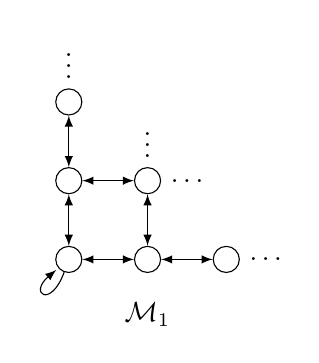
\begin{tikzpicture}[>=latex]

  \node (n11) at (0,0) [shape=circle,draw] {} edge [in=220, out=250,loop] ();
  \node (n22) at (1,1) [shape=circle,draw, label=right:$\dots$, label=above:$\vdots$] {};
  \node (n12) at (0,1) [shape=circle,draw] {} ;
  \node (n21) at (1,0) [shape=circle,draw] {};
  \node (n13) at (0,2) [shape=circle,draw, label=above:$\vdots$] {};
  \node (n31) at (2,0) [shape=circle,draw, label=right:$\dots$] {};

  \draw [<->] (n11) -- (n12);
  \draw [<->] (n21) -- (n22);
  \draw [<->] (n12) -- (n22);
  \draw [<->] (n11) -- (n21);
  \draw [<->] (n21) -- (n31);
  \draw [<->] (n12) -- (n13);

  \node at (1,-.7) {$\mathcal{M}_1$};

\end{tikzpicture}
\hspace{10mm}
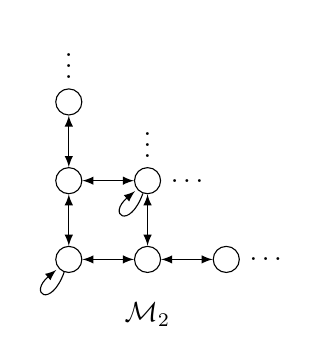
\begin{tikzpicture}[>=latex]

  \node (n11) at (0,0) [shape=circle,draw] {}
                       edge [in=220, out=250,loop] ();
  \node (n22) at (1,1) [shape=circle,draw, label=right:$\dots$, label=above:$\vdots$] {}
                       edge [in=220, out=250,loop] ();
  \node (n12) at (0,1) [shape=circle,draw] {} ;
  \node (n21) at (1,0) [shape=circle,draw] {};
  \node (n13) at (0,2) [shape=circle,draw, label=above:$\vdots$] {};
  \node (n31) at (2,0) [shape=circle,draw, label=right:$\dots$] {};

  \draw [<->] (n11) -- (n12);
  \draw [<->] (n21) -- (n22);
  \draw [<->] (n12) -- (n22);
  \draw [<->] (n11) -- (n21);
  \draw [<->] (n21) -- (n31);
  \draw [<->] (n12) -- (n13);

  \node at (1,-.7) {$\mathcal{M}_2$};
\end{tikzpicture}
\end{center}

%\begin{center}
%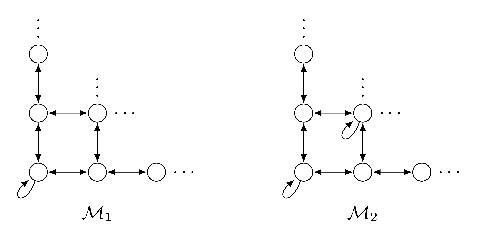
\includegraphics[scale=0.8]{figure1.eps}
%\medskip
\caption{Two \tle-bisimilar models}\label{fig}
\end{figure}

We prove that $\model_1,0\bisim\model_2,0$
showing the winning strategy for duplicator. Intuitively, the strategy for Duplicator consists in the following idea: whenever one player is in $(\model_1,0)$ the other will be in $(\model_2,0)$ or $(\model_2,1)$, and
conversely whenever a player is in $(\model_1,n)$, $n>0$ the other will be in
$(\model_2,m)$, $m>1$. This is maintained until Spoiler (if ever) decides to
remember a state. Once this is done, then any strategy will be a winning one for Duplicator.


Being a bit more formal, the winning strategy will have two stages. While Spoiler does not remember any reflexive
state, Duplicator plays with the following strategy: if Spoiler
chooses $0$ in any model, Duplicator chooses $0$ in the other one;
if Spoiler chooses $n>0$ in $\model_1$, Duplicator plays $n+1$ in
$\model_2$; if Spoiler chooses $n>0$ in $\model_2$, Duplicator plays
$n-1$ in $\model_1$.

Notice that with this strategy Spoiler chooses
a reflexive state if and only if Duplicator answers with a reflexive
one. This is clearly a winning strategy. If ever Spoiler decides to
remember a reflexive state, Duplicator starts using the following
strategy: if Spoiler selects a state $n$, Duplicator answers with an
agreeing state $m$ of the opposite model. Notice that this is always
possible since both $n$ and $m$ see infinitely many non remembered
states and at least one remembered state. Therefore $\model_1,w \bisim \model_2, w$.

On the other hand, let $\varphi$ be the formula $\down i. \diam{r}(i \land \diam{r}(\lnot i \land \down i.\diam{r}i))$. It is easy to see that $\model_1, w \not \models \varphi$ but $\model_2, w \models \varphi$.
\end{pf}

The basic idea behind the previous proof is that if the relations
$R_1$ and $R_2$ extend the set $\{(n,m) \mid n\not= m\}$, then
$\tle$ can distinguish between irreflexive and non irreflexive frames,
but it cannot distinguish frames with a different number of reflexive nodes.

There is a number of interesting remarks to be made above the
previous proof. First, notice that it is essential for the winning
strategy of Duplicator that each state in a model is related to
infinitely many others.


We have already shown that $\tle \not= \hlogic$ and we used a pair
of infinite models to distinguish both logics. We now analyze the
question whether $\tle \not= \hlogic$ on image-finite models. We
prove that $\hlogic \not \leq \tle$ on image-finite models showing
that there cannot exist an equivalence preserving translation for
finite models from $\hlogic$ to $\tle$

\tb{below should not be a definition (it is only used in the proof of Theorem 10).
Give first the theorem and move the lemmas to 'claims' within the proof.  The
definition of the models goes also inside the proof.}

\begin{defn}
Let $\model^1_n = \diam{W_n, R_1, \emptyset, \emptyset}$ and
$\model^2_n = \diam{W_n, R_2, \emptyset, \emptyset}$, where
$W_n=\{w_0, \dots, w_{n-1}\}$, $R_1 = \{(n,m)\mid n \neq m\} \cup
\{(w_0,w_0)\}$ and $R_2 = \{(n,m)\mid n \neq m\} \cup \{(w_0,w_0)\}
\cup \{w_1, w_1\}$, with $n\geq 1$.
\end{defn}

\begin{lem}\label{lem:not-distinguish}
Let $\varphi$ be a $\tle$-formula such that the number of
occurrences of the $\remember$ operator is at most $n$. Then
$\model^1_{n+2}, w_0 \models \varphi$ iff $\model^2_{n+2}, w_0
\models \varphi$.
\end{lem}

\begin{pf}
We prove that Duplicator has a winning strategy in the game
$E(\model^1_{n+2},\model^2_{n+2}, w_0, w_0)$ in the case Spoiler
makes at most $n$ memorizing steps. The strategy for Duplicator is
the following. While Spoiler does not remember any reflexive state,
Duplicator plays with the following strategy: if Spoiler chooses
$w_0$ in any model, Duplicator chooses $w_0$ in the other one; if
Spoiler chooses $w_k$, $0 < k < n+1$, in $\model_1$, Duplicator
plays $w_{k+1}$ in $\model_2$, and if Spoiler chooses $w_{n+1}$ in
$\model_1$, Duplicator plays $w_2$ in $\model_2$; if Spoiler chooses
$w_k$, $k > 0$, in $\model_2$, Duplicator plays $w_{k-1}$ in
$\model_1$. Note that with this strategy, Spoiler chooses a
reflexive state iff Duplicator answers with a reflexive one. If ever
Spoiler decides to remember a reflexive state, then from that point
of the game, for every state $w_n$ chosen by Spoiler, Duplicator
will always have an agreeing state $w_m$ on the opposite model he
can choose. This happens because the models have $n+2$ states, and
therefore there is always at least two non-remembered states. That
means that both $w_n$ and $w_m$ see at least one remembered state
and at least one non-remembered state, and this condition will hold
for the rest of the game.
\end{pf}

\begin{lem}\label{lem:distinguish}
Let $\varphi = \down i. \diam{R}(i \land \diam{R}(\lnot i \land
\down i. \diam{R}i))$. For every $n \geq 1$, $\model^1_n, w_0
\not\models \varphi$ and $\model^2_n, w_0 \models \varphi$.
\end{lem}
\begin{pf}
Trivial.
\end{pf}

\begin{thm}
There is no translation $Tr$ from $\hlogic$-sentences to
$\tle$-formulas such that for every finite model $\model$ and every
formula $\varphi$ of $\hlogic$ we have $\model \models_{\hlogic}
\varphi$ iff $\model \models_{\tle} Tr(\varphi)$.
\end{thm}
\begin{pf}
Let us suppose that such translation $Tr$ exists. Let $\varphi$ a
$\hlogic$-formula as in Lemma~\ref{lem:distinguish}, and let $n$ be
the complexity of $Tr(\varphi)$. Because $Tr(\varphi)$ has at most
$n$ remember operators, we know by Lemma~\ref{lem:not-distinguish}
that $\model^1_{n+2}, w_0 \models Tr(\varphi)$ iff $\model^2_{n+2},
w_0 \models Tr(\varphi)$. But on the other hand, $\model^1_{n+2},
w_0 \not \models \varphi$ and $\model^2_{n+2}, w_0 \models \varphi$.
This is an absurd, since $Tr$ should be an equivalence preserving
translation for finite models.
\end{pf}




Second, notice that the $\hlogic$ sentence that we used in the proof
uses only one nominal.  Hence, we have actually proved that
$\hlogicone\not\le\tle$, where $\hlogicone$ is $\hlogic$ restricted
to only one nominal.  But actually, it is also the case that $\tle
\not\le\hlogicone$.

\tb{Give the general claim for an arbitrary $k$ as a theorem. Then
say that we just prove the case for $k=1$ and that the rest are similar.}
\begin{pro}\label{prop:hlogicone_incomparable_tle}
The logics $\hlogicone$ and {\em $\tle$} are incomparable in terms of expressive power.
\end{pro}

\begin{pf}
As we said, $\hlogicone\not\leq\tle$ is a direct consequence of the
proof of Theorem~\ref{thm:tle_not_equal_hlogic}. To prove $\tle \not
\le \hlogicone$, let $\model_1=\diam{\{1,2,3\},\{(i,j) \mid 1 \leq
i,j \leq 3\},\emptyset,\emptyset}$ (a clique of size 3) and
$\model_2=\diam{\{1,2\},\{(i,j) \mid 1 \leq i,j \leq
2\},\emptyset,\emptyset}$ (a clique of size 2). It is easy to check
that $\model_1,1 \bisim_{\hlogicone} \model_2,1$. However, the
formula
$\varphi = \remember \diam{r} (\neg \known \land \remember
\diam{r} (\neg\known \land \remember \diam{r} \neg\known))$
distinguishes the models: $\model_1,1 \models \varphi$ but
$\model_2,1 \not\models \varphi$.
\end{pf}

Actually, this incomparability result can be extended to $\hlogic$ restricted to any fixed number of nominals, by taking cliques of the appropriate size.

\begin{thm}
For any fixed $k$, the logics $\hlogick$ and {\em $\tle$} are incomparable in terms of expressive power.
\end{thm}
\medskip

\noindent
We will now briefly discuss the case of $\tl$.  As we already mentioned at the beginning
of this section, the first required step to compare expressivity is to be able to define
a natural mapping between models of the different logics involved.  Consider a model
$\diam{W,\rels,V,S}$ for $\tl$; if we want to associate a Kripke model we have to decide
how to deal with the set $S$.  The only natural choice seems to be to extend the signature
with a special propositional variable \emph{known}, and let $V'$ be identical to
$V$ excepts that $V'(\mathit{known}) = S$.  And  the same can be done to obtain a hybrid model
from a $\tl$ model.


\begin{thm}\label{thm:expr_power}
The following results concerning expressive power can be established
\begin{enumerate}
\item $\bml$ over the signature $\diam{\prop \cup \{\mathit{known}\}, \rel}$ is strictly
less expressive than {\em $\tl$} over the signature $\diam{\prop, \rel}$.
\item {\em $\tl$} over the signature $\diam{\prop, \rel}$ is strictly less expressive
than $\hlogic$ over the signature $\diam{\prop \cup \{\mathit{known}\}, \rel,\nom}$.
\item {\em $\tle$} over the signature $\diam{\prop \cup \{\mathit{known}\}, \rel}$ is equivalent to \linebreak
{\em $\tl$} over the signature $\diam{\prop, \rel}$
\end{enumerate}
\end{thm}

\begin{pf}
All proofs are similar to (and sometimes easier than) the ones
presented above. We only discuss 2. To prove $\tl \le \hlogic$ (over
the appropriate signatures) we adapt the translation $\Tr$ with the
following clause for $\known$
$$
\begin{array}{rcl}
\Tr_N(\known) & = & \big (\bigvee_{i \in N} i \big) \vee
\mathit{known}.
\end{array}
$$
$\hlogic \not \le \tl$ can be shown using the following models. Let
$\model_1=\diam{\{w\},$ $\{(w,w)\},\emptyset,\{w\}}$ and
$\model_2=\diam{\{u,v\},\{(u,v),(v,u)\},\emptyset,\{u,v\}}$.
Duplicator always wins on $E(\model_1,\model_2,w,u)$ and thus
$\model_1,w\bisim_{\tl}\model_2,u$. On the other hand,
$\model'_1,w\models_{\hlogic}\down i.\diam{r}i$ but
$\model'_2,u\not\models_{\hlogic}\down i.\diam{r}i$, for $\model'_1,
\model'_2$ the  models corresponding to $\model_1$ and $\model_2$.
\end{pf}

\begin{pro}\label{prop:stack_leq_hl}
$\MS$ is not more expressive than $\hlogic$.
\end{pro}

\begin{pf}
We show that every property captured by a $\MS$-formula can be
captured by a $\hlogic$-formula. We do this by defining the
following translation transforming an $\MS$-formula and a list of
nominals $N$ into an $\hlogic$-formula.
\begin{eqnarray*}
\Tr_N(p) & = & p \quad p \in \prop\\
\Tr_N(\lnot \varphi) & = & \lnot \Tr_N(\varphi) \\
\Tr_N(\diam{r} \varphi) & = & \diam{r} \Tr_N(\varphi) \\
\Tr_N(\varphi_1 \land \varphi_2) & = & \Tr_N(\varphi_1) \land \Tr_N(\varphi_2)\\
\Tr_N(\push \varphi) & = & \down i. \Tr_{N\cdot i}(\varphi) \quad
\textrm{where $i \notin N$.}\\
\Tr_{N\cdot i}(\pop \varphi) & = & \Tr_{N}(\varphi)\\
\Tr_{[\ ]}(\pop \varphi) & = & \lnot\top\\
\Tr_{N\cdot i}(\tope) & = & i\\
\Tr_{[\ ]}(\tope) & = & \lnot\top
\end{eqnarray*}
(Here $q$ is a fixed propositional symbol in \prop.)

It can be shown by induction in $\varphi$ that $\model, w \models
\varphi$ iff $\model, g, w \models \Tr_{[\ ]}(\varphi)$, for any $g$
\end{pf}

\begin{pro} \label{prop:hl_leq_stack}
$\hlogic$ is not more expressive than $\MS$.
\end{pro}

\begin{pf}
As in the previous proof, we define a translation transforming an
$\hlogic$-formula and a list of nominals $N$ into an $\MS$-formula.
The idea is that in a formula of the form $\down i.\down j.\varphi$
we can stack first $i$ and then $j$. Now if $i$ and $j$ appear in
$\varphi$, then $j$ must be translated as $\tope$ and  $i$ must be
translated as $\pop\tope$. We define the translation which coincides
with the one defined in the proof of
Proposition~\ref{prop:stack_leq_hl} for the propositional, negation,
conjunction and modality, plus:
\begin{eqnarray*}
\Tr_N(\down i.\varphi) & = & \push\Tr_{N\cdot i}(\varphi)\\
\Tr_N(i) & = & \pop^{\len{N}-x}\tope \quad i \in \nom, N[x]=i,
\forall y>x:\, N[y]\not=i
\end{eqnarray*}
(Here $\len{N}$ represents the length of $N$; for convenience the
lists are numbered from $1$ and $N[x]$ represents the $x$-th element
of $N$.)

It can be shown by induction in $\varphi$ that if $\varphi$ is an
$\hlogic$-formula with no free nominals, $\model, g, w \models
\varphi$ iff $\model, w \models \Tr_{[\ ]}(\varphi)$ for any $g$.
\end{pf}

\begin{cor}
$\MS$ and $\hlogic$ have the same expressive power.
\end{cor}

To close this section, we mention that the satisfaction preserving translations defined in
the proof can actually be used to transfer known results, for example, from  $\hlogic$ to $\tl$ and $\tle$.  For
instance, both logics are compact and their formulas are preserved by generated submodels (see~\cite{areces01:_hybrid}).

\section{(Un)Decidability and the Finite Model Property}

In Section~\ref{expressivity} we show four memory logics ($\cMLRK$,
$\cMLRKE$, $\cMLRKM$ and $\cMLRKME$) which are all more expressive
than $\bml$ but less expressive than $\hlogic$. Given that $\bml$ is
decidable and $\hlogic$ is undecidable, exploring where the
decidability line lies is an intriguing question.  The main goal of
this section is to investigate this issue, together with the related
question of whether the language is sufficiently expressive to force
infinite models.

We start by investigating $\cMLRKM$ and $\cMLRKME$. We will show
that even though they are equivalent in terms of expressive power
when we allow a shift if the signature, the satisfiability problem
for $\cMLRKM$ is decidable (actually \textsc{pspace}-complete) while
$\cMLRKME$ is already undecidable. As we will show in the proof of
Theorem~\ref{thm:fmp} the trick will be to use a `dirty' memory. In
$\cMLRKME$, we are restricted to the class of models where the
memory is always initialized to $\emptyset$ and we can't play this
trick anymore.  Actually $\cMLRKM$ is really standing on the
decidability line, adding a single nominal to $\cMLRKM$ push the
satisfiability problem over to undecidability.

\subsection{The Decidability of $\cMLRKM$\ldots}

We will first prove that $\bml$ and $\cMLRKM$ expressively
equivalent over the class of tree-like models.  With that result
at hand, we will then prove that $\cMLRKM$ has a tree model
property, and from that decidability and \textsc{pspace}-completeness
follows.

\begin{thm}\label{prop:sat-preserv-tree}
$\K$  over the signature $\tup{\prop \cup \{\mathit{known}\},\rel}$
is equivalent to $\cMLRKM$ over the class of tree models.
\end{thm}

\begin{pf}
$[\K \le \cMLRKM]$: This is a direct corollary of Theorem~\ref{teo:bml_ml}.
\smallskip

\noindent
$[\cMLRKM \le \K]$: %
% We first define, given a formula
% $\varphi$, a new formula More formally:
%
% \begin{displaymath}\label{sharp}
% \begin{array}{rcl}
% p^\sharp & = & p \quad p \in \prop\\
% \known^\sharp & = & \top \\
% (\lnot \varphi)^\sharp & = & \lnot \varphi^\sharp \\
% (\varphi_1 \land \varphi_2)^\sharp & = & \varphi_1^\sharp \land \varphi_2^\sharp \\
% (\remember \varphi)^\sharp & = & \remember \varphi^\sharp\\
% (\ttup{r} \varphi)^\sharp & = & \ttup{r} \varphi
% \end{array}
% \end{displaymath}
We start by noticing that in $\cMLRKM$ we can eliminate
$\known$ at modal depth 0 from a formula like $\remember \varphi$.

\begin{claim}\label{lem:replace}
Let $\varphi^\sharp$ be the result of replacing all the occurrences
of $\known$ that are in $\varphi \in \cMLRKM$ at modal depth zero by $\top$. Then $\model, w \models \remember
\varphi$ iff $\model, w \models \varphi^\sharp$.
\end{claim}

\begin{pfclaim}
We proceed by induction on $\varphi$. The case for $\known$, the propositional
symbols and booleans are straightforward. We analyze the other
cases:
\begin{itemize}
 \item $\varphi = \remember \psi$. $\model, w \models \remember\remember\psi$ iff $\model, w \models \remember \psi$ iff (by inductive hypothesis) $\model, w \models \psi^\sharp$ iff $\model, w \models (\psi^\sharp)^\sharp$ iff (by inductive hypothesis) $\model, w \models \remember (\psi^\sharp)$ iff $\model, w \models (\remember\psi)^\sharp$
\item $\varphi = \ttup{r} \psi$. $\model, w \models \remember \ttup{r} \psi$ iff (by definition) $\model[w], w \models \ttup{r} \psi$ iff (by definition of $\sharp$) $\model[w], w \models (\ttup{r} \psi)^\sharp$ iff (by definition) $\model, w \models (\ttup{r} \psi)^\sharp$
\end{itemize}
\end{pfclaim}

Define now the following translation taking $\cMLRKM$ formulas over the signature
$\diam{\prop, \rel}$ to $\bml$-formulas over the signature
$\diam{\prop \cup \{known\}, \rel}$:
$$
\begin{array}{rcl}
\Tr(p) & = & p \quad p \in \prop\\
\Tr(\known) & = & known \\
\Tr(\lnot \varphi) & = & \lnot \Tr(\varphi) \\
\Tr(\varphi_1 \land \varphi_2) & = & \Tr(\varphi_1) \land \Tr(\varphi_2) \\
\Tr(\ttup{r} \varphi) & = & \diam{r} \Tr(\varphi) \\
\Tr(\remember \varphi) & = & \Tr(\varphi^\sharp)
\end{array}
$$

Let $\varphi \in \cMLRKM$, and let $\gM=\tup{W,\rels,V,S}$ be an arbitrary tree
model.  Let $\gM'=\tup{W,\rels,V'}$ where $V'$ is identical to $V$ except that
$V'(\mathit{known})=S$. We can prover that $\gM,w \models \varphi \mbox{ iff } \gM',w \models \Tr(\varphi)$.

We proceed by induction on $\varphi$. The propositional and boolean
cases are trivial. The $\known$ case is also easy given the
definitions. For the diamond case. Given that $\gM$ is tree-like,
the remember operator has no effect beyond modal operators, so
$\gM, w \models \ttup{r}\psi$ iff exists $v$ such that
$R(w,v)$ and $\gM,v\models \psi$. By inductive hypothesis,
$\gM',v\models \psi$ iff $\gM', v \models
\Tr(\psi)$, and by definition $\gM', w \models \diam{r}
\Tr(\psi)$. Finally, let's see the case for remember. By
Claim~\ref{lem:replace}, $\gM, w \models \remember \psi$
iff $\gM, w \models \psi^\sharp$. By inductive hypothesis,
$\gM, w \models \Tr(\psi^\sharp)$.
\end{pf}





%\subsection{Finite model property}

% \begin{lem}\label{lem:frontera-k}
% Let $\model$ be a model and $w \in \model$. Then $(\model
% \upharpoonright n),w \bisim_n \model, w$.
% \end{lem}
%
% \begin{pf}
% In the game $E_n(\model, \model \upharpoonright n, w, w)$ the
% winning strategy for Duplicator consists in copying Spoiler moves.
% This can always be done because Spoiler cannot go beyond $n$ steps
% from $w$.
% \end{pf}

% \begin{thm}
% Let $\model$ be a model and $w \in \model$. For every $n \geq 0$,
% $\model, w \leftrightsquigarrow_n (\model \upharpoonright n), w$.
% \end{thm}
%
% \begin{pf}
% This result follows from Theorem~\ref{thm:bisim-n-to-prune} and
% Theorem~\ref{thm:bisim-tlm-n-to-modal-n}.
% \end{pf}

We now prove that $\cMLRKM$ has the \emph{tree model property}~\cite{BRV01},
that is, every satisfiable formula in $\cMLRKM$ is satisfied in a tree model.

\begin{thm}[Tree model property]\label{prop:tree-model-property}
For every $\cMLRKM$-model
$\model$ and $w\in\model$ there is a tree-like model $\model'$ where
$w\in\model'$ and $\tup{\model,w}\equiv^\EF\tup{\model',w}$.
\end{thm}

\begin{pf}
Let $\model=\diam{W,R,V,S}$.  We prove the result for the unimodal
case, the generalization to the multimodal case is straightforward.
We define the model $\model'=\diam{W',R',V',S'}$ as follows. Its
domain $W'$ consists on all finite sequences $(u_0,\dots,u_n)$ such
that $u_0=w$, $n\geq 0$ and there is a path $u_0Ru_1\dots Ru_n$ in
$\model$. Define $(u_0,\dots,u_n)R(v_0,\dots,v_m)$ to hold if
$m=n+1$, $u_i=v_1$ for $i=0,\dots,n$ and $u_nRv_m$ holds in
$\model$. The valuation $V'$ is defined by setting
$(u_0,\dots,u_n)\in V'(p)$ iff $u_n\in V(p)$. Finally,
$(u_0,\dots,u_{n-1},u_n)\in S'$ iff $u_n\in\{u_0,\dots,u_{n-1}\}$ or
$u_n\in S$.

We call $s_i$ the sequence $(v_0,\dots,v_i)$ for every
$i=0,\dots,n$. Let us see that Duplicator has a winning strategy in
the game $\EF(\model,\model',w,w)$. It is sufficient to see that in
the game
$\EF(\model[v_0,\dots,v_n],\model'[s_0,\dots,s_n],v_{n+1},s_{n+1})$,
Duplicator can always answer successfully to Spoiler's move.
\begin{itemize}
\item
If Spoiler chooses $\model[v_0,\dots,v_n]$ and some $v_{n+1}$, a
successor of $v_n$, Duplicator chooses the sequence
$s_{n+1}=s_nv_{n+1}$.

\item
If Spoiler chooses $\model'[s_0,\dots,s_n]$ and $s_{n+1}=s_nv_{n+1}$
(for some $v_{n+1}$), a successor of $s_n$, Duplicator chooses the
state $v_{n+1}$.
\end{itemize}

By definition, it is easy to see that $s_{n+1}$ and $v_{n+1}$ agree.
Observe that at this stage of the game the current ``memory" of
$\model[v_0,\dots,v_n]$ is $S \cup \{v_0,\dots,v_n\}$ and the
current ``memory" of $\model'[s_0,\dots,s_n]$ is $S' \cup
\{s_0,\dots,s_n\}$. Then it is also clear that $v_{n+1}$ was
remembered at this stage of the game, if and only if $s_{n+1}$ also
was. More formally, on the one hand, $v_{n+1}\in S \cup
\{v_0,\dots,v_n\}$ implies $s_{n+1} \in S'$ by definition. On the
other hand if $s_{n+1}\in S' \cup \{s_0,\dots,s_n\}$, we have
$s_{n+1}\in S'$ (since there are no cycles in $\model'$) and by
definition $v_{n+1}\in S \cup \{v_0,\dots,v_n\}$.
\end{pf}

%If $\model$ is a $\cMLRKM$-model, we denote with $\model_T$ the
%tree-like model constructed in the above proposition.

%\begin{lem}\label{lem:bisim_bml_then_bisim_tlm}
%Let $\model,\nodel$ be two $\tlm$ tree-like models. For any $n$, if
%the equivalent $\bml$-models satisfy
%$\model,w\bisim_n^{\bml}\nodel,v$ then
%$\model,w\bisim_n^{\tlm}\nodel,v$.
%\end{lem}
%
%\begin{pf}
%Let $\model=\diam{W_1,R_1,V_1,S_1}$ and
%$\nodel=\diam{W_2,R_2,V_2,S_2}$.
%%
%Recall the definition of $n$-bisimulation for $\bml$
%\cite[Definition 2.30]{BRV01}, involving the relations
%$Z_0\supseteq\dots\supseteq Z_{n}$. We define a winning strategy for
%Duplicator in terms of $Z_0,\dots,Z_{n}$.
%
%We start in the game $E(\model,\nodel,w,v)$. We show that if
%$E(\model',\nodel',w',v')$ is some $i$th stage of that game ($i\leq
%n$) and $w'Z_{n-i}v'$, then for any choice $u$ of Spoiler,
%Duplicator can always answer with $t$ such that $uZ_{n-i-1}t$.
%Suppose Spoiler chooses $u\in\model'$ such that $w'Ru$. By
%definition of $Z_{n-i}$, there exists $t\in\nodel'$ such that $v'Rt$
%and $vZ_{n-i-1}t$. It follows from the definition of $Z_0$ that $u$
%and $t$ agree. Observe that the game $E(\model',\nodel',w',v')$ is
%just equivalent to $E(\model,\nodel,w',v')$, since both $\model$ and
%$\nodel$ are acyclic. Therefore $u\in S_1$ iff $t\in S_2$. The case
%Spoiler chooses to play in $\nodel'$ is similar and this completes
%the proof.
%\end{pf}

%\begin{thm}\label{thm:fmp-tlm}
%Let $\model$ be a model. For every $n$ there is a finite tree-like
%model $\nodel$ such that $\model\bisim_n\nodel$.
%\end{thm}

%\begin{pf}
%By Proposition~\ref{prop:tree-model-property},
%$\model\bisim^{\tlm}\model_T$. By
%Theorem~\ref{thm:bisim-n-to-prune},
%$\model_T\bisim_n^{\tlm}\model_T\upharpoonright n$. Applying the
%selection process in \cite[Theorem 2.34]{BRV01} on the equivalent
%$\bml$-model for $\model_T\upharpoonright n$ we obtain  a finite
%tree-like model $\nodel$ such that $\model_T\upharpoonright
%n\bisim_n^{\bml}\nodel$. Applying
%Lemma~\ref{lem:bisim_bml_then_bisim_tlm}, we know that
%$\model_T\upharpoonright n\bisim_n^{\tlm}\nodel$ and therefore
%$\model \bisim_n^{\tlm}\nodel$.
%\end{pf}

\begin{thm}\label{thm:fmp}
The satisfiability problem of $\cMLRKM$ is \pspace-complete.
\end{thm}

\begin{pf}
We first show decidability of the satisfiability problem of 
$\cMLRKM$ proving that any satisfiable formula of $\cMLRKM$ is satisfiable in a
recursively bounded model.

Let $\varphi$ be a $\cMLRKM$ formula of degree $k$, and suppose
$\gM_1,w \models \varphi$. By
Theorem~\ref{prop:tree-model-property}, there is a tree-like
model $\gM_2$ such that $\gM_2,w \models \varphi$.
Using Theorem~\ref{prop:sat-preserv-tree}, we know that $\gM_2',w \models
\Tr(\varphi)$. Now we can use the \emph{finite} tree model property for
basic modal logic~\cite{BRV01}, so there must be a recursively bounded tree-like
model $\gM_3=\tup{W,\rels,V}$ and $v \in W$ such that $\gM_3,v \models \Tr(\varphi)$.
Finally, we can use Theorem~\ref{prop:sat-preserv-tree} again,
and conclude $\tup{W,\rels,V,V(\mathit{known})},v \models \varphi$.
% 
% Observe that it is known~\cite{BRV01} that $\gM_3$ has at most
% $n^k$ states, where $n$ is the number of non-equivalent formulas of
% degree at most $k$, containing the same propositional symbols of
% $\varphi$.

The \pspace-completeness follows from the fact that the translation 
$\Tr$ is linear.
\end{pf}


%\begin{cor}[Finite model property]
%If $\varphi\in\tlm$ is satisfiable then it is satisfiable on a
%finite model.
%\end{cor}

%\begin{thm}[Alternative proof for the finite model property] (without using Lemma~\ref{lem:bisim_bml_then_bisim_tlm})
%If $\varphi\in\tlm$ is satisfiable then it is satisfiable on a
%finite model.
%\end{thm}
%\begin{pf}
%Let $\varphi$ be a $\tlm$ formula, and suppose $\model,w \models
%\varphi$. By Proposition~\ref{prop:tree-model-property}, there is a
%tree-like model $\model'$ such that $\model',w \models \varphi$.
%Using Proposition~\ref{prop:sat-preserv-tree}, we can turn to basic
%modal logic $\bml$, and assert that $\model',w \models_{\bml}
%Tr(\varphi)$. Now we can use the finite tree model property for
%basic modal logic \cite{??}, so there must be a finite tree-like
%model $\model''$ such that $\model'',w \models_{\bml} Tr(\varphi)$.
%Finally, we can use Proposition~\ref{prop:sat-preserv-tree} again,
%and conclude $\model'',w \models \varphi$.
%\end{pf}

% \begin{thm}
% The satisfaction problem for $\cMLRKM$ is -complete.
% \end{thm}
% \begin{pf}
% The lower \textsc{pspace}-hard bound for $\cMLRKM$ follows from the
% lower bound for the basic modal logic~\cite{BRV01}. We show a
% matching upper bound by reducing the satisfiability problem for
% basic modal logic. Given a $\cMLRKM$-formula $\varphi$, we compute
% $\Tr(\varphi)$ as in the proof of Theorem~\ref{prop:sat-preserv-tree}. Note that the
% size of the translated formula $\Tr(\varphi)$ is actually at most
% the size of $\varphi$. Let suppose that $\Tr(\varphi)$ has a model,
% that is $\model, w \models_{\bml} \Tr(\varphi)$. This happens iff
% there exists a tree-like model $\model'$ such that $\model', w
% \models_{\bml} \Tr(\varphi)$ (by the tree model property of $\bml$)
% iff $\model', w \models_{\cMLRKM} \varphi$ (by
% Proposition~\ref{prop:sat-preserv-tree}) iff there exists a model
% $\nodel$ such that $\nodel,w \models_{\cMLRKM} \varphi$ (by the tree
% model property for $\cMLRKM$, stated in
% Proposition~\ref{prop:tree-model-property}). Therefore, given
% $\varphi$, determining the $\bml$-satisfiability of $\Tr(\varphi)$
% (and we can do this with a \textsc{pspace} algorithm~\cite{BRV01})
% is enough to decide the $\cMLRKM$-satisfiability of $\varphi$.
% \end{pf}

\subsection{\ldots and its Undecidable Neighbours}

We now show the undecidability of two variations of $\cMLRKM$.

While $\cMLRKM$ is decidable, it seems to be standing at the 
border of undecidability.  The logic $\cMLRKME$, obtained from $\cMLRKM$ by 
restricting the class of models to those where $S=\emptyset$ is
undecidable.  Actually, adding one single nominal to $\cMLRKM$ 
already leads to undecidability.

Let's call $\cMLRKM + i$ the logic obtained by extending 
$\cMLRKM$ with a single nominal. We first prove failure of
the finite model property for $\cMLRKM + i$.

\begin{thm}\label{thm:tlmi:inf}
$\cMLRKM + i$ lacks the finite model property.
\end{thm}

\begin{pf}
Consider the following formulas:
$$
\begin{array}{rl}
(\textit{Back}) & i \land \bbox{r}\lnot i  \land \ttup{r} \top \land \bbox{r}\ttup{r} i \\
%&$``The root is irreflexive, and in symmetric relation with all its (nonempty) successors.''$\\
(\textit{Empty}) & \bbox{r}\lnot \known \land \bbox{r}\bbox{r}(\lnot i \to \lnot \known)\\
%&$``One step and two steps successors are not known.''$\\
(\textit{Spy}) & \bbox{r}\bbox{r}( \lnot i \to \ttup{r} (i \land \ttup{r} ( \known \land \lnot \ttup{r} ( \known \land \lnot i))))\\
%&$``All successors are irreflexive.''$\\
%(\textit{Irr}) & \lnot \ttup{r} \ttup{r} ( \lnot i \land \known))\\
(\textit{Succ}) & \bbox{r}\ttup{r} \lnot i \\
(\textit{no-3cyc}) & \lnot \ttup{r} \ttup{r} ( \lnot \known \land \ttup{r} ( \lnot \known \land \ttup{r} ( \known \land \lnot i)))\\
(\textit{Tran}) & \bbox{r} \ttup{r} ( i \land \bbox{r} ( \lnot \known \to \ttup{r}( i \land \ttup{r} ( \known \land  \ttup{r}(\known \land \lnot i) ))))\\
\end{array}
$$
%
Let $\textit{Inf}$ be $\textit{Back} \land \textit{Empty} \land
\textit{Spy} \land \textit{Irr} \land \textit{Succ} \land
\textit{3cyc} \land \textit{Tran}$. Let $\model=\diam{W, R, V,
\emptyset}$. Let us see that if $\model, w \models \textit{Inf}$,
then $W$ is infinite.
%
Suppose $\model, w \models \textit{Inf}$. Let $B = \{b \in W \mid
wRb\}$. Because $\textit{Back}$ is satisfied, $w \not \in B$, $B
\not= \emptyset$ and for all $b \in B$, $bRw$. Note that
\textit{Empty} says that the one and two-step horizon is not known,
and also this implies that every state in $B$ is irreflexive.
Because $\textit{Spy}$ is satisfied, if $a \not= w$ and $a$ is a
successor of an element of $B$ then $a$ is also an element of $B$.
As $\textit{Succ}$ is satisfied at $w$, every point in $B$ has a
successor distinct from $w$. As $\textit{no-3cyc}$ is satisfied,
there cannot be $3$ different elements in $B$ forming a cycle, and
this sentence together with $\textit{Tran}$ force $R$ to
transitively order $B$.
%
It follows that $B$ is an unbounded strict partial order as showed in the picture below, hence infinite, and so is $W$.
\begin{center}
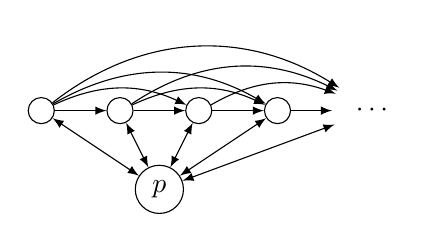
\begin{tikzpicture}[>=latex]
  \node (n1) at (1.5,.5) [shape=circle,draw] {$p$} ;
  \node (n2) at (0,1.5) [shape=circle,draw] {} ;
  \node (n3) at (1,1.5) [shape=circle,draw] {} ;
  \node (n4) at (2,1.5) [shape=circle,draw] {} ;
  \node (n5) at (3,1.5) [shape=circle,draw] {} ;
  \node (n6) at (4.2,1.5) [shape=circle, minimum height=1cm] {$\cdots$} ;

  \draw [<->] (n1) -- (n2);
  \draw [<->] (n1) -- (n3);
  \draw [<->] (n1) -- (n4);
  \draw [<->] (n1) -- (n5);
  \draw [<->] (n1) -- (n6);
  
  \draw [->] (n2) -- (n3);
  \draw [->] (n3) -- (n4);
  \draw [->] (n4) -- (n5);
  \draw [->] (n5) -- (n6);
  
  \draw [->] (n2) edge[bend left=25] (n4);
  \draw [->] (n3) edge[bend left=25] (n5);
  \draw [->] (n4) edge[bend left=25] (n6);
  
  \draw [->] (n2) edge[bend left=30] (n5);
  \draw [->] (n3) edge[bend left=30] (n6);
  
  \draw [->] (n2) edge[bend left=35] (n6);
\end{tikzpicture}
\end{center}

\end{pf}


We now show that this logic is undecidable by encoding the
$\omega\times\omega$ tiling problem (see~\cite{BGG97}). Following
the idea in~\cite{BS95}, we construct a spy point over the relation
$s$ which has access to every tile. The relations $u$ and $r$
represent moving up and to the right, respectively, from one tile to
the other. We code each type of tile with a fixed propositional
symbol $t_i$. With this encoding we define for each tiling problem
$T$, a formula $\varphi^T$ such that the set of tiles $T$ tiles
$\omega\times\omega$ iff $\varphi^T$ has a model.


\begin{thm}\label{thm:tlmi:und}
The satisfiability problem for $\cMLRKM + i$ is undecidable.
\end{thm}
\begin{pf}
Let $T=\{T_1,\dots,T_n\}$ be a set of tile types. Given a tile type
$T_i$, $u(T_i)$, $r(T_i)$, $d(T_i)$, $l(T_i)$ will represent the
colors of the up, right, down and left edges of $T_i$ respectively.
Define:
$$
\begin{array}{rl}
(\textit{Back}) & i \land \bbox{s}\lnot i \land \ttup{s} \top \land \bbox{s}\ttup{s}i \land \bbox{s}\bbox{s}i\\
(\textit{Empty}) & \bbox{s}\lnot \known \land \bbox{s}\bbox{s}(\lnot i \to \lnot \known) \land \bbox{s}[\dag]\lnot \known \quad \dag \in \{r,u\}\\
(\textit{Spy}) & \bbox{s}[\dag]\ttup{s}(i \land \ttup{s}(\known \land \lnot\diam{\dag}\known)) \quad \dag \in \{r,u\}\\
(\textit{Grid}) & \bbox{s}\diam{\dag} \top \quad \dag \in \{r,u\}\\
(\textit{Func}) & \bbox{s}[\dag]\ttup{s}\ttup{s}(\known \land \diam{\dag}\known \land [\dag]\known) \quad \dag \in \{r,u\}\\
(\textit{Conf}) & \bbox{s}\ttup{u}\ttup{r}\ttup{s}\ttup{s}(\known \land \lnot \ttup{r}\known \land \ttup{u}\known \land \\
& \ \ \ \ttup{r}( \lnot \known \land (\ttup{u}(\known \land \lnot \ttup{r}\known)))\\
(\textit{UR-no-Cycle}) & \bbox{s}\bbox{u}\bbox{r}\lnot \known \land \bbox{s}\bbox{r}\bbox{u}\lnot \known\\
(\textit{URU-no-Cycle}) & \bbox{s}\bbox{u}\bbox{r}\bbox{u}\lnot \known\\
(\textit{Unique}) & \bbox{s} \left( \bigvee_{1\leq i\leq n} t_i \wedge \bigwedge_{1\leq i < j \leq n } (t_i\to \lnot t_j)\right) \\
(\textit{Vert}) & \bbox{s} \bigwedge_{1\leq i\leq n} \left( t_i \to \ttup{u} \bigvee_{1\leq j\leq n,u(T_i)=d(T_j)}  t_j\right) \\
(\textit{Horiz}) & \bbox{s} \bigwedge_{1\leq i\leq n} \left( t_i \to \ttup{r} \bigvee_{1\leq j\leq n,r(T_i)=l(T_j)}  t_j\right) \\
\end{array}
$$

Let the formula $\varphi^T$ be the conjunction of all the above
formulas. We show that $T$ tiles $\omega\times\omega$ iff
$\varphi^T$ is satisfiable.

Suppose $\model,w\models\varphi^T$. Observe that (\textit{Back}) and
(\textit{Spy}), together with (\textit{Empty}) impose $w$ to be a
spy point over all its $S$-accessible states of $\model$ (and also
force $U$ and $R$ to be irreflexive and asymmetric). These
$S$-accessible states will be the tiles. From this it follows that
$[s]\psi$ holds at $w$ iff $\psi$ is true at every tile.
Additionally, $\diam{s}\diam{s}\psi$ holds at tile $v$ iff $\psi$ is
true at some tile (maybe the same one).

Taking the above points into account, one can establish the
following. (\textit{Grid}) states that from every tile there is
another tile moving up (that is, following the $U$-relation). The
same holds for the right direction (following the $R$-relation).
(\textit{Func}) forces that $U$ and $R$ are both functionals, given
that (\textit{Back}) and (\textit{Spy}) guarantee irreflexivity and
asymmetry of $U$ and $R$ respectively. (\textit{Conf}) imposes that
the tiles are arranged in a grid pattern. To make its job,
(\textit{Conf}) needs the composed relation $U\circ R$ to be
irreflexive, and to avoid a cycle with the $URU$ pattern. This job
is done by (\textit{UR-Irr}) and (\textit{URU-noCycle})
respectively.

All the formulas we discuss up to now configure the grid. The last
three ensure that every tile has a unique type $t_i$, and that the
colors of the tiles match properly. From this, it easily follows
that $\model$ is a tiling of $\omega\times\omega$.

For the converse, suppose $f:\omega\times\omega\to T$ is a tiling of
$\omega\times\omega$. We define the model
$\model=\diam{W,\{S,U,R\},V,\emptyset}$ as follows:
\begin{itemize}
\item $W=\omega\times\omega \cup \{w\}$
\item $S=\{(w,v),(v,w)\mid v\in\omega\times\omega\}$  (hence $w$ will act as the spy
point)
\item $U=\{((x,y),(x,y+1))\mid x,y\in\omega\}$
\item $R=\{((x,y),(x+1,y))\mid x,y\in\omega\}$
\item $V(p)=\{w\}$; $V(t_i)=\{x\mid x\in\omega\times\omega, f(x)=T_i\}$
\end{itemize}
The reader may verify that, by construction,
$\model,w\models\varphi^T$.
\end{pf}

We now turn to the case for $\cMLRKME$.


\begin{thm}\label{thm:tlme:inf}
$\cMLRKME$ lacks the finite model property.
%
%There is a formula $\textit{Inf} \in \cMLRKME$ such that
%$\mathcal{M},w \models \textit{Inf}$ implies that the domain of
%$\mathcal{M}$ is an infinite set.
\end{thm}

\begin{pf}
Consider the following formulas:
$$
\begin{array}{rl}
(\textit{Back}) & p \land \bbox{r} \lnot p  \land \ttup{r} \top \land \bbox{r}\ttup{r} (\known \land p) \\
%&$``The root is irreflexive, and in symmetric relation with all its (nonempty) successors.''$\\
(\textit{Spy}) & \bbox{r}\bbox{r}( \lnot p \to \ttup{r} (\known \land p \land \ttup{r} ( \known \land \lnot \ttup{r} ( \known \land \lnot p))))\\
%&$``A 2-step successor is a 1-step successor, with a non-symmetric relation between them.''$\\
(\textit{Irr}) & \lnot \ttup{r} ( \lnot p \land \ttup{r} ( \lnot p \land \known)))\\
%&$``All successors are irreflexive.''$\\
(\textit{Succ}) & \bbox{r}\ttup{r} \lnot p \\
%&$``All successors have a successor different from the root.''$\\
(\textit{no-3cyc}) & \lnot \ttup{r}   \ttup{r} ( \lnot \known \land \ttup{r} ( \lnot \known \land \ttup{r} ( \known \land \lnot p)))\\
%&$``There are no cycles of 3 elements between successors of the root.''$\\
(\textit{Tran}) & \bbox{r} ( \lnot p \to \ttup{r} ( \known \land p \land \bbox{r} ( \lnot p \land \lnot \known \to \ttup{r}( \known \land p \land \\
& \ \ \ \ttup{r} ( \known \land \lnot p \land  \ttup{r}(\known \land \lnot p) )))))\\
%&$``Every pair of successors $u$ and $v$ are related (either $uRv$ or $vRu$).''$\\
\end{array}
$$

Let $\textit{Inf}$ be $\textit{Back} \land \textit{Spy} \land
\textit{Irr} \land \textit{Succ} \land \textit{no-3cyc} \land
\textit{Tran}$. Let $\model=\diam{W, R, V, \emptyset}$. One can
follow the idea used in the proof of Theorem~\ref{thm:tlmi:inf} to
show that if $\model, w \models \textit{Inf}$, then $\model$ is
infinite.

In that proof, the use of $i$ was to identify the spy point. We now
don't have nominals, but using $S=\emptyset$, we can replace $i$
with a clever combination of a propositional symbol $p$ and
$\known$. Since we want to univocally identify the spy point and $p$
may hold in many states, sometimes we need to use $\known$ to
distinguish which one is the spy point (in the proof of
Theorem~\ref{thm:tlmi:inf}, this was not necessary because the
nominal $i$ is true at only one state).

Notice that \textit{Back}, \textit{Spy}, \textit{Succ}, and
\textit{no-3cyc} are very similar to the ones in the proof of
Theorem~\ref{thm:tlmi:inf}, \textit{Irr} forces $R$ to be
irreflexive and \textit{Tran} says that every pair of successors $u$
and $v$ are related (either $uRv$ or $vRu$), and this together with
the other formulas, implies that $R$ is transitive.

%
%Suppose $\model, w \models \textit{Inf}$. Let $B = \{b \in W \mid
%wRb\}$. Because $\textit{Back}$ is satisfied, $w \not \in B$, $B
%\not= \emptyset$ and for all $b \in B$, $bRw$. Because
%$\textit{Spy}$ is satisfied, if $a \not= w$ and $a$ is a successor
%of an element of $B$ then $a$ is also an element of $B$. As
%$\textit{Irr}$ is satisfied at $w$, every state in $B$ is
%irreflexive. As $\textit{Succ}$ is satisfied at $w$, every point in
%$B$ has a successor distinct from $w$. As $\textit{3cyc}$ is
%satisfied, there cannot be $3$ different elements in $B$ forming a
%cycle, and this sentence together with $\textit{Tran}$ force $R$ to
%transitively order $B$.
%
%It follows that $B$ is an unbounded strict partial order, hence
%infinite, and so is $W$.
\end{pf}


In the same way as before, we now show that the satisfiability
problem for $\cMLRKME$ is undecidable, by encoding the $\omega
\times \omega$ tiling problem.

\begin{thm}\label{thm:tlme:und}
The satisfiability problem for $\cMLRKME$ is undecidable.
\end{thm}
\begin{pf}
Let $T=\{T_1,\dots,T_n\}$ be a set of tile types. Given a tile type
$T_i$, $u(T_i)$, $r(T_i)$, $d(T_i)$, $l(T_i)$ will represent the
colors of the up, right, down and left edges of $T_i$ respectively.
Define:
$$
\begin{array}{rl}
(\textit{Back}) & p \land \bbox{s}\lnot p \land \ttup{s} \top \land \bbox{s}\ttup{s}(\known \land p) \land \bbox{s}\bbox{s}(\known \land p)\\
(\textit{Spy}) & \bbox{s}[\dag](\lnot p \land \ttup{s}(\known \land p \land \ttup{s}(\known \land \lnot\diam{\dag}\known))) \quad \dag \in \{r,u\}\\
(\textit{Grid}) & \bbox{s}\diam{\dag} \top \quad \dag \in \{r,u\}\\
(\textit{Func}) & \bbox{s}[\dag]\ttup{s}\ttup{s}(\known \land \diam{\dag}\known \land [\dag]\known) \quad \dag \in \{r,u\}\\
(\textit{Conf}) & \bbox{s}\ttup{u}\ttup{r}\ttup{s}\ttup{s}(\known \land
\lnot \ttup{r}\known \land \ttup{u}\known \land \\
& \ \ \ \ttup{r}\ttup{u}(\known \land \lnot \ttup{r}\known))\\
(\textit{URU-no-Cycle}) & \bbox{s}\bbox{u}\bbox{r}\lnot \known \land \bbox{s}\bbox{r}\bbox{u}\lnot \known\\
(\textit{URU-no-Cycle}) & \bbox{s}\bbox{u}\bbox{r}\bbox{u}\lnot \known\\
(\textit{Unique}) & \bbox{s} \left( \bigvee_{1\leq i\leq n} t_i \wedge \bigwedge_{1\leq i < j \leq n } (t_i\to \lnot t_j)\right) \\
(\textit{Vert}) & \bbox{s} \bigwedge_{1\leq i\leq n} \left( t_i \to \ttup{u} \bigvee_{1\leq j\leq n,u(T_i)=d(T_j)}  t_j\right) \\
(\textit{Horiz}) & \bbox{s} \bigwedge_{1\leq i\leq n} \left( t_i \to
\ttup{r} \bigvee_{1\leq j\leq n,r(T_i)=l(T_j)}  t_j\right)
\end{array}
$$

Let the formula $\varphi^T$ be the conjunction of all the above
formulas. One can show that $T$ tiles $\omega\times\omega$ iff
$\varphi^T$ is satisfiable, following the ideas used in the proof of
Theorem~\ref{thm:tlmi:und} and the observation in the proof of
Theorem~\ref{thm:tlme:inf}.

%Suppose $\model,w\models\varphi^T$. Observe that (\textit{Back}) and
%(\textit{Spy}) impose $w$ to be a spy point over all its
%$S$-accessible states of $\model$ (and also force $U$ and $R$ to be
%irreflexive and asymmetric). These $S$-accessible states will be the
%tiles. From this it follows that $[S]\psi$ holds at $w$ iff $\psi$
%is true at every tile. Additionally, $\diam{S}\diam{S}\psi$ holds at
%tile $v$ iff $\psi$ is true at some tile (maybe the same one).
%
%Taking the above points into account, one can establish the
%following. (\textit{Grid}) states that from every tile there is
%another tile moving up (that is, following the $U$-relation). The
%same holds for the right direction (following the $R$-relation).
%(\textit{Func}) forces that $U$ and $R$ are both functionals, given
%that (\textit{Back}) and (\textit{Spy}) guarantee irreflexivity and
%asymmetry of $U$ and $R$ respectively. (\textit{Conf}) imposes that
%the tiles are arranged in a grid pattern. To make its job,
%(\textit{Conf}) needs the composed relation $U\circ R$ to be
%irreflexive, and to avoid a cycle with the $URU$ pattern. This job
%is done by (\textit{UR-Irr}) and (\textit{URU-noCycle})
%respectively.
%
%All the formulas we discuss up to now configure the grid. The last
%three ensure that every tile has a unique type $t_i$, and that the
%colors of the tiles match properly. From this, it easily follows
%that $\model$ is a tiling of $\omega\times\omega$.
%
%For the converse, suppose $f:\omega\times\omega\to T$ is a tiling of
%$\omega\times\omega$. We define the model
%$\model=\diam{W,\{S,U,R\},V,\emptyset}$ as follows:
%\begin{itemize}
%\item $W=\omega\times\omega \cup \{w\}$
%\item $S=\{(w,v),(v,w)\mid v\in\omega\times\omega\}$  (hence $w$ will act as the spy
%point)
%\item $U=\{((x,y),(x,y+1))\mid x,y\in\omega\}$
%\item $R=\{((x,y),(x+1,y))\mid x,y\in\omega\}$
%\item $V(p)=\{w\}$; $V(t_i)=\{x\mid x\in\omega\times\omega, f(x)=T_i\}$
%\end{itemize}
%The reader may verify that, by construction,
%$\model,w\models\varphi^T$.
%
\end{pf}

\subsection{The Undecidables $\cMLRK$ and $\cMLRKE$}

From the undecidability of $\cMLRKME$, we can easily conclude the
undecidability of $\cMLRK$ and $\cMLRKE$.

\begin{thm}
$\cMLRKE$ lacks the finite model property and is undecidable.
\end{thm}

\begin{pf}
Straightforward from the effective translation given as a result of $\cMLRKME \leq \cMLRKE$
(Theorem~\ref{thm:four-le-two}) and theorems~\ref{thm:tlme:inf}
and~\ref{thm:tlme:und}.
\end{pf}

To prove failure of the finite model property for the case $\cMLRK$
we first notice that the following lemma is easy to establish (we only
state it for the mono-modal case; a similar result is true in the
multi-modal case).
Failure of the finite model property is then a direct consequence.

\begin{lem}\label{lem:boxes}
Let $\varphi$ be a formula of modal depth $d$. If
{\em $\diam{W,R_r,V,S},w\models$} \linebreak {\em $\left(\bigwedge_{i=0}^d [r]^i \lnot
\known\right) \wedge \varphi$} then $\diam{W,R_r,V,\emptyset},w\models
\varphi$.
\end{lem}

\begin{cor}
{\em $\cMLRK$} lacks the finite model property.
\end{cor}

\begin{pf}
Using Lemma~\ref{lem:boxes}, one can easily see that the formula
$\textit{Inf}\land \left(\bigwedge_{i=0}^4 [r]^i \lnot
\known\right)$, where $\textit{Inf}$ is the one in the proof of
Theorem~\ref{thm:tlme:inf}, forces an infinite model.
\end{pf}



\begin{cor}
The satisfiability problem for {\em $\cMLRK$} is undecidable.
\end{cor}
%
\begin{pf}
Using the idea of Lemma~\ref{lem:boxes} and the formula $\varphi^T$
in the proof of Theorem~\ref{thm:tlme:und}, we can obtain a formula
$\psi$ such that if $\model,w\models\psi$ then $\model$ is a tiling
of $\omega \times \omega$. For the converse, we can build exactly
the same model as in the proof of Theorem~\ref{thm:tlme:und} and
check that it satisfies $\psi$.
\end{pf}

%\section{A decidable fragment}

%\begin{defn}[Syntax]\label{syntax}
%Let $\prop=\{p_1, p_2, \dots\}$ (the \textit{propositional symbols})
%and $\rel=\{r_1, r_2, \dots\}$ (the \textit{relational symbols}) be
%pairwise disjoint, countable infinite sets of symbols. The set
%$\forms$ of formulas of $\tlm$ in the signature $\langle
%\prop,\rel\rangle$ is defined as:
%$$
%\forms ::= p \mid \known \mid \lnot \varphi \mid \varphi_1 \land
%\varphi_2 \mid \diam{R} \varphi \mid \remember \varphi,
%$$
%where $p \in \prop$, $R \in \rel$  and $\varphi, \varphi_1,
%\varphi_2 \in \forms$.
%\end{defn}



In this section we study another member of the memory logics family,
called $\tlm$, in which the behavior of the \emph{remember} operator
is highly coupled with the modal transitions. In this logic, every
time we make a modal step, we are constrained to remember the
current state. We change the semantic definition of $\diam{r}$ to
be:
$$
\begin{array}{rcl}
\diam{W,\rels,V,S}, w \models \diam{r} \varphi & \iff & \exists w' \in W, R_r(w,w') \textrm{ and } \\
& & \diam{W,\rels,V, S \cup \{w\}}, w' \models \varphi
\end{array}
$$
We will show how this change in the semantic of $\diam{r}$ leads to
some interesting results.

We define the \textit{Ehrenfucht game} $\game$ for $\tlm$ in the
same way as for $\tl$, with the following modifications: in step 2,
Spoiler always remembers the current world, and the game goes on
with $E(\model_1[w_1], \model_2[w_2], v_1, v_2)$ after Duplicator
response.

%We define bisimulation and $n$-bisimulation between models
%($\model_1 \bisim \model_2$ and $\model_1 \bisim_n \model_2$) in the
%same way as before. In particular, note that Theorem~\ref{bisim} and
%\ref{thm:hennesy} hold for $\tlm$.
%
%SACAR LOS TEOREMAS Y SOLO HACER REFERENCIA A LOS QUE YA TENEMOS
%
%\begin{thm}
%Let $\model_1, \model_2$ be two models, $w_1 \in \model_1, w_2 \in
%\model_2$. If $w_1 \bisim w_2$ then $w_1 \leftrightsquigarrow w_2$.
%\end{thm}
%
%\begin{thm}
%Let $\model_1, \model_2$ be two image finite models. Then for every
%$w_1 \in \model_1$ and $w_2 \in \model_2$,  $w_1 \bisim w_2$ iff
%$w_1 \leftrightsquigarrow w_2$.
%\end{thm}


%\begin{defn}[$n$-Bisimulation]
%We say that two models $\model_1$ and $\model_2$ are $n$-bisimilar
%($\model_1 \bisim_n \model_2$) when there exists $w_1 \in \model_1$
%and $w_2 \in \model_2$ such that they agree in the same
%propositional symbols and Duplicator has a winning strategy on
%$E_n(\model_1, \model_2, w_1, w_2)$. In this case we will also say
%that $w_1$  and $w_2$ are $n$-bisimilar ($\model_1, w_1 \bisim_n
%\model_2, w_2$).
%\end{defn}
%
%FALTA DEFINIR $E_n$ Y $EQUIV_n$
%
%\begin{thm}\label{thm:bisim-n-to-modal-n}
%Let $\model_1,\model_2$ be two models, $w_1 \in \model_1, w_2 \in
%\model_2$. If $w_1 \bisim_n w_2$ then $w_1 \leftrightsquigarrow_n
%w_2$.
%\end{thm}
%
%\begin{pf}
%The proof can be done by induction on $n$.
%\end{pf}
%
%For a natural number $k$, the restriction of a model $\model$ to $k$
%(notation: $\model \upharpoonright k$) is defined as the submodel
%containing only states whose height is at most $k$.
%
%
%\begin{thm}\label{thm:bisim-n-to-prune}
%Let $\model$ be a model and $w \in \model$. For every $n \geq 0$,
%$\model, w \bisim_n (\model \upharpoonright n), w$.
%\end{thm}
%
%\begin{pf}
%It is easy to see that in an $n$-round game the players only visit
%states with height at most $n$ and thus, as far as the players are
%concerned, $\model$ and $\model\upharpoonright n$ are the same.
%Therefore Duplicator can always copy Spoiler's moves.
%\end{pf}
%
%
%% \begin{pf}
%% We follow the same idea as in Theorem~\ref{bisim}. The only non
%% trivial case is $\varphi = \diam{R} \psi$. We prove that
%% $\model_1,w_1 \models \diam{R} \psi$ implies $\model_2,w_2 \models
%% \diam{R} \psi$. Suppose $\model_1,w_1 \models \diam{R} \psi$. Then
%% there is $v_1\in \model_1$ such that $w_1R_1v_1$ and
%% $\model_1[w_1],v_1\models\psi$. Suppose that Spoiler chooses model
%% $\model_1$ at step 1 and $v_1$ as an $R_1$-successor. By
%% Lemma~\ref{lem:strategy}, Duplicator has a winning winning strategy
%% on $E(\model_1[w_1], \model_2[w_2], w_1, w_2)$, and following that
%% strategy, he finds $v_2$ such that $\props(v_1)=\props(v_2)$,
%% $w_2R_2v_2$, and keeps a winning strategy on $E(\model_1[w_1],
%% \model_2[w_2], v_1, v_2)$. By inductive hypothesis and the fact that
%% $\model_1[w_1],v_1\models\psi$, we conclude
%% $\model_2[w_2],v_2\models\psi$ and therefore
%% $\model_2,w_2\models\diam{R} \psi$. The other direction is
%% identical.
%% \end{pf}


We now give some results related to the expressive power of $\tlm$.

\begin{thm}
$\bml$ over the signature $\diam{\prop \cup \{known\}, \rel}$ is
strictly less expressive than $\tlm$ over the signature
$\diam{\prop, \rel}$.
\end{thm}

\begin{pf}
Exactly the same proof used to prove that $\bml < \tl$.
\end{pf}

\begin{thm}
$\tlm < \tl$.
\end{thm}

\begin{pf}
It is easy to see that there is a translation from $\tlm$ to $\tl$
which maps $\diam{R}\varphi$  to  $\remember\diam{R}\varphi$. To see
that the inclusion is strict, let $\model_1=\diam{\{w,v,r\}, R_1,
V_1, \emptyset}$ and $\model_2=\diam{\{w,v,r\}, R_2, V_2,
\emptyset}$ such that $R_1=\{(w,v),(v,r),(r,w)\}$,
$R_2=\{(w,v),(v,r),(r,v)\}$ and $V_1(p) = V_2(p) = \emptyset$ for
all $p \in \prop$.
% \begin{center}
% \begin{pgfpicture}{0cm}{0cm}{4cm}{1cm}
%     \pgfnodecircle{nodo1}[stroke]{\pgfxy(0.5,0.5)}{0.25cm}
%     \pgfnodecircle{nodo2}[stroke]{\pgfxy(2.0,0.5)}{0.25cm}
%     \pgfnodecircle{nodo3}[stroke]{\pgfxy(3.5,0.5)}{0.25cm}
%
%     \pgfsetlinewidth{0.4pt}
%     \pgfnodesetsepstart{1.5pt}
%     \pgfnodesetsepend{3pt}
%     \pgfsetendarrow{\pgfarrowtriangle{4pt}}
%     \pgfnodeconnline{nodo1}{nodo2}
%     \pgfnodeconnline{nodo2}{nodo3}
% %    \pgfnodeconncurve{nodo3}{nodo1}{225}{315}{1cm}{1cm}
%
%     \pgfnodelabel{nodo1}{nodo1}[-17][0pt]{\pgfbox[center,base]{$w$}}
%     \pgfnodelabel{nodo3}{nodo3}[-30][1.5cm]{\pgfbox[center,base]{$\model_1$}}
% \end{pgfpicture}
% \hspace{20mm}
% \begin{pgfpicture}{0cm}{0cm}{4cm}{1cm}
%     \pgfnodecircle{nodo1}[stroke]{\pgfxy(0.5,0.5)}{0.25cm}
%     \pgfnodecircle{nodo2}[stroke]{\pgfxy(2.0,0.5)}{0.25cm}
%     \pgfnodecircle{nodo3}[stroke]{\pgfxy(3.5,0.5)}{0.25cm}
%
%     \pgfsetlinewidth{0.4pt}
%     \pgfnodesetsepstart{1.5pt}
%     \pgfnodesetsepend{3pt}
%     \pgfsetendarrow{\pgfarrowtriangle{4pt}}
%     \pgfnodeconnline{nodo1}{nodo2}
%     \pgfnodeconnline{nodo2}{nodo3}
% %    \pgfnodeconncurve{nodo3}{nodo2}{225}{315}{0.2cm}{1cm}
%
%     \pgfnodelabel{nodo1}{nodo1}[-17][0pt]{\pgfbox[center,base]{$w$}}
%     \pgfnodelabel{nodo3}{nodo3}[-30][1.5cm]{\pgfbox[center,base]{$\model_2$}}
% \end{pgfpicture}
% \vspace{8mm}
% \end{center}
We prove that $\model_1$ and $\model_2$ are $\tlm$-bisimilar. As
every state in both models has a unique successor, Duplicator has
only one way of playing, and this only way is indeed a winning
strategy. From this follows that no formula in $\tlm$ can
distinguish $\model_1$ and $\model_2$. On the other hand, let
$\varphi = \diam{R}\remember\diam{R}\diam{R}\known$ be a
$\tl$-formula. It is easy to see that $\model_1,w \not \models
\varphi$, but $\model_2, w \models \varphi$.
\end{pf}

We now establish an equivalence result between $\bml$ and $\tlm$ for
the class of tree-like models. We first define, given a formula
$\varphi$, a new formula $\varphi^\sharp$, as the result of
replacing all the ocurrences of $\known$ that are in $\varphi$ at
modal depth zero by $\top$. More formally:

\begin{displaymath}\label{sharp}
\begin{array}{rcl}
p^\sharp & = & p \quad p \in \prop\\
\known^\sharp & = & \top \\
(\lnot \varphi)^\sharp & = & \lnot \varphi^\sharp \\
(\varphi_1 \land \varphi_2)^\sharp & = & \varphi_1^\sharp \land \varphi_2^\sharp \\
(\remember \varphi)^\sharp & = & \remember \varphi^\sharp\\
(\diam{R} \varphi)^\sharp & = & \diam{R} \varphi
\end{array}
\end{displaymath}


\begin{lem}\label{lem:replace}
$\model, w \models \remember \varphi$ iff $\model, w \models
\varphi^\sharp$.
\end{lem}

\begin{pf}
We proceed by induction. The case for $\known$, the propositional
symbols and booleans are straightforward. We analyze the other
cases:
\begin{itemize}
 \item $\varphi = \remember \psi$. $\model, w \models \remember\remember\psi$ iff $\model, w \models \remember \psi$ iff (by inductive hypothesis) $\model, w \models \psi^\sharp$ iff $\model, w \models (\psi^\sharp)^\sharp$ iff (by inductive hypothesis) $\model, w \models \remember (\psi^\sharp)$ iff $\model, w \models (\remember\psi)^\sharp$
\item $\varphi = \diam{R} \psi$. $\model, w \models \remember \diam{R} \psi$ iff (by definition) $\model[w], w \models \diam{R} \psi$ iff (by inductive hypothesis) $\model[w], w \models (\diam{R} \psi)^\sharp$ iff (by definition) $\model, w \models (\diam{R} \psi)^\sharp$
\end{itemize}
\end{pf}

We are now ready to define an equivalence preserving translation for
the tree-like models.

\begin{defn}[Translation]\label{def:tr-tlm-k}
Let $known$ be a new proposition symbol not in $\prop$. The
translation $\Tr$, taking $\tlm$ formulas over the signature
$\diam{\prop, \rel}$ to $\bml$-formulas over the signature
$\diam{\prop \cup \{known\}, \rel}$ is defined as:

\begin{displaymath}
\begin{array}{rcl}
\Tr(p) & = & p \quad p \in \prop\\
\Tr(\known) & = & known \\
\Tr(\lnot \varphi) & = & \lnot \Tr(\varphi) \\
\Tr(\varphi_1 \land \varphi_2) & = & \Tr(\varphi_1) \land \Tr(\varphi_2) \\
\Tr(\diam{R} \varphi) & = & \diam{R} \Tr(\varphi) \\
\Tr(\remember \varphi) & = & \Tr(\varphi^\sharp)
\end{array}
\end{displaymath}

\end{defn}

Taking the same model equivalence used to compare $\bml$ with $\tl$,
the following result can be established:

\begin{pro}[Satisfiability preserving]\label{prop:sat-preserv-tree}
Let $\model$ be a a tree-like model. Then
$\model,w\models_{\tlm}\varphi$ iff $\model,w\models_{\bml}
\Tr(\varphi)$.
\end{pro}

\begin{pf}
We proceed by induction on $\varphi$. The propositional and boolean
cases are trivial. The $\known$ case is also easy given the
definitions. For the diamond case. Given that $\model$ is tree-like,
the remember operator has no effect beyond modal operators, so
$\model, w \models_{\tlm} \diam{R}\psi$ iff exists $v$ such that
$wRv$ and $\model,v\models_{\tlm} \psi$. By inductive hypothesis,
$\model,v\models_{\tlm} \psi$ iff $\model, v \models_{\bml}
\Tr(\psi)$, and by definition $\model, w \models_{\bml} \diam{R}
\Tr(\psi)$. Finally, let's see the case for remember. By
Lemma~\ref{lem:replace}, $\model, w \models_{\tlm} \remember \psi$
iff $\model, w \models_{\tlm} \psi^\sharp$. By inductive hypothesis,
$\model, w \models_{\bml} \Tr(\psi^\sharp)$.
\end{pf}



%\subsection{Finite model property}

% \begin{lem}\label{lem:frontera-k}
% Let $\model$ be a model and $w \in \model$. Then $(\model
% \upharpoonright n),w \bisim_n \model, w$.
% \end{lem}
%
% \begin{pf}
% In the game $E_n(\model, \model \upharpoonright n, w, w)$ the
% winning strategy for Duplicator consists in copying Spoiler moves.
% This can always be done because Spoiler cannot go beyond $n$ steps
% from $w$.
% \end{pf}

% \begin{thm}
% Let $\model$ be a model and $w \in \model$. For every $n \geq 0$,
% $\model, w \leftrightsquigarrow_n (\model \upharpoonright n), w$.
% \end{thm}
%
% \begin{pf}
% This result follows from Theorem~\ref{thm:bisim-n-to-prune} and
% Theorem~\ref{thm:bisim-tlm-n-to-modal-n}.
% \end{pf}



\begin{pro}[Tree model
property]\label{prop:tree-model-property} For every $\tlm$-model
$\model$ and $w\in\model$ there is a tree-like model $\model'$ where
$w\in\model'$ and $\model,w\bisim\model',w$.
\end{pro}

\begin{pf}
Let $\model=\diam{W,R,V,S}$.  We prove the result for the unimodal
case, the generalization to the multimodal case is straightforward.
We define the model $\model'=\diam{W',R',V',S'}$ as follows. Its
domain $W'$ consists on all finite sequences $(u_0,\dots,u_n)$ such
that $u_0=w$, $n\geq 0$ and there is a path $u_0Ru_1\dots Ru_n$ in
$\model$. Define $(u_0,\dots,u_n)R(v_0,\dots,v_m)$ to hold if
$m=n+1$, $u_i=v_1$ for $i=0,\dots,n$ and $u_nRv_m$ holds in
$\model$. The valuation $V'$ is defined by setting
$(u_0,\dots,u_n)\in V'(p)$ iff $u_n\in V(p)$. Finally,
$(u_0,\dots,u_{n-1},u_n)\in S'$ iff $u_n\in\{u_0,\dots,u_{n-1}\}$ or
$u_n\in S$.

We call $s_i$ the sequence $(v_0,\dots,v_i)$ for every
$i=0,\dots,n$. Let us see that Duplicator has a winning strategy in
the game $E(\model,\model',w,w)$. It is sufficient to see that in
the game
$E(\model[v_0,\dots,v_n],\model'[s_0,\dots,s_n],v_{n+1},s_{n+1})$,
Duplicator can always answer successfully to Spoiler's move.
\begin{itemize}
\item
If Spoiler chooses $\model[v_0,\dots,v_n]$ and some $v_{n+1}$, a
successor of $v_n$, Duplicator chooses the sequence
$s_{n+1}=s_nv_{n+1}$.

\item
If Spoiler chooses $\model'[s_0,\dots,s_n]$ and $s_{n+1}=s_nv_{n+1}$
(for some $v_{n+1}$), a successor of $s_n$, Duplicator chooses the
state $v_{n+1}$.
\end{itemize}
By definition, it is easy to see that $s_{n+1}$ and $v_{n+1}$ agree.
Observe that at this stage of the game the current ``memory" of
$\model[v_0,\dots,v_n]$ is $S \cup \{v_0,\dots,v_n\}$ and the
current ``memory" of $\model'[s_0,\dots,s_n]$ is $S' \cup
\{s_0,\dots,s_n\}$. Then it is also clear that $v_{n+1}$ was
remembered at this stage of the game, if and only if $s_{n+1}$ also
was. More formally, on the one hand, $v_{n+1}\in S \cup
\{v_0,\dots,v_n\}$ implies $s_{n+1} \in S'$ by definition. On the
other hand if $s_{n+1}\in S' \cup \{s_0,\dots,s_n\}$, we have
$s_{n+1}\in S'$ (since there are no cycles in $\model'$) and by
definition $v_{n+1}\in S \cup \{v_0,\dots,v_n\}$.
\end{pf}

If $\model$ is a $\tlm$-model, we denote with $\model_T$ the
tree-like model constructed in the above proposition.

%\begin{lem}\label{lem:bisim_bml_then_bisim_tlm}
%Let $\model,\nodel$ be two $\tlm$ tree-like models. For any $n$, if
%the equivalent $\bml$-models satisfy
%$\model,w\bisim_n^{\bml}\nodel,v$ then
%$\model,w\bisim_n^{\tlm}\nodel,v$.
%\end{lem}
%
%\begin{pf}
%Let $\model=\diam{W_1,R_1,V_1,S_1}$ and
%$\nodel=\diam{W_2,R_2,V_2,S_2}$.
%%
%Recall the definition of $n$-bisimulation for $\bml$
%\cite[Definition 2.30]{BRV01}, involving the relations
%$Z_0\supseteq\dots\supseteq Z_{n}$. We define a winning strategy for
%Duplicator in terms of $Z_0,\dots,Z_{n}$.
%
%We start in the game $E(\model,\nodel,w,v)$. We show that if
%$E(\model',\nodel',w',v')$ is some $i$th stage of that game ($i\leq
%n$) and $w'Z_{n-i}v'$, then for any choice $u$ of Spoiler,
%Duplicator can always answer with $t$ such that $uZ_{n-i-1}t$.
%Suppose Spoiler chooses $u\in\model'$ such that $w'Ru$. By
%definition of $Z_{n-i}$, there exists $t\in\nodel'$ such that $v'Rt$
%and $vZ_{n-i-1}t$. It follows from the definition of $Z_0$ that $u$
%and $t$ agree. Observe that the game $E(\model',\nodel',w',v')$ is
%just equivalent to $E(\model,\nodel,w',v')$, since both $\model$ and
%$\nodel$ are acyclic. Therefore $u\in S_1$ iff $t\in S_2$. The case
%Spoiler chooses to play in $\nodel'$ is similar and this completes
%the proof.
%\end{pf}

%\begin{thm}\label{thm:fmp-tlm}
%Let $\model$ be a model. For every $n$ there is a finite tree-like
%model $\nodel$ such that $\model\bisim_n\nodel$.
%\end{thm}

%\begin{pf}
%By Proposition~\ref{prop:tree-model-property},
%$\model\bisim^{\tlm}\model_T$. By
%Theorem~\ref{thm:bisim-n-to-prune},
%$\model_T\bisim_n^{\tlm}\model_T\upharpoonright n$. Applying the
%selection process in \cite[Theorem 2.34]{BRV01} on the equivalent
%$\bml$-model for $\model_T\upharpoonright n$ we obtain  a finite
%tree-like model $\nodel$ such that $\model_T\upharpoonright
%n\bisim_n^{\bml}\nodel$. Applying
%Lemma~\ref{lem:bisim_bml_then_bisim_tlm}, we know that
%$\model_T\upharpoonright n\bisim_n^{\tlm}\nodel$ and therefore
%$\model \bisim_n^{\tlm}\nodel$.
%\end{pf}

\begin{thm}
If $\varphi\in\tlm$ is satisfiable then it is satisfiable on a
finite model.
\end{thm}

\begin{pf}
Let $\varphi$ be a $\tlm$ formula, and suppose $\model,w \models
\varphi$. By Proposition~\ref{prop:tree-model-property}, there is a
tree-like model $\model'$ such that $\model',w \models \varphi$.
Using Proposition~\ref{prop:sat-preserv-tree}, we can turn to basic
modal logic $\bml$, and assert that $\model',w \models_{\bml}
Tr(\varphi)$. Now we can use the finite tree model property for
basic modal logic \cite{??}, so there must be a finite tree-like
model $\model''$ such that $\model'',w \models_{\bml} Tr(\varphi)$.
Finally, we can use Proposition~\ref{prop:sat-preserv-tree} again,
and conclude $\model'',w \models \varphi$.
\end{pf}


%\begin{cor}[Finite model property]
%If $\varphi\in\tlm$ is satisfiable then it is satisfiable on a
%finite model.
%\end{cor}

%\begin{thm}[Alternative proof for the finite model property] (without using Lemma~\ref{lem:bisim_bml_then_bisim_tlm})
%If $\varphi\in\tlm$ is satisfiable then it is satisfiable on a
%finite model.
%\end{thm}
%\begin{pf}
%Let $\varphi$ be a $\tlm$ formula, and suppose $\model,w \models
%\varphi$. By Proposition~\ref{prop:tree-model-property}, there is a
%tree-like model $\model'$ such that $\model',w \models \varphi$.
%Using Proposition~\ref{prop:sat-preserv-tree}, we can turn to basic
%modal logic $\bml$, and assert that $\model',w \models_{\bml}
%Tr(\varphi)$. Now we can use the finite tree model property for
%basic modal logic \cite{??}, so there must be a finite tree-like
%model $\model''$ such that $\model'',w \models_{\bml} Tr(\varphi)$.
%Finally, we can use Proposition~\ref{prop:sat-preserv-tree} again,
%and conclude $\model'',w \models \varphi$.
%\end{pf}


\begin{cor}[Decidability]\label{cor:tlm-decidability}
$\tlm$ is decidable.
\end{cor}

\begin{pf}
Given $\varphi$ with modal degree $k$, it suffices to observe that
in the selection process (in the proof of
Theorem~\ref{thm:fmp-tlm}), one can bound the number of elements of
the constructed model by $n^k$, where $n$ is the number of
non-equivalent formulas of degree at most $k$, containing the same
propositional symbols of $\varphi$. Therefore, to decide the
satisfiability of $\varphi$ one can check if $\model\models\varphi$
for all models $\model$ with size at most $n^k$.
\end{pf}

\begin{thm}[\mbox{\rm\textsc{pspace}}-complete]
The satisfaction problem for $\tlm$ is \textsc{pspace}-complete.
\end{thm}
\begin{pf}
The lower \textsc{pspace}-hard bound for $\tlm$ follows from the
lower bound for the basic modal logic~\cite{BRV01}. We show a
matching upper bound by reducing the problem to the satisfiability
problem for basic modal logic. Given a $\tlm$-formula $\varphi$, we
compute $\Tr(\varphi)$ using Definition~\ref{def:tr-tlm-k}. Note
that the size of the translated formula $\Tr(\varphi)$ is actually
smaller than $\varphi$. Let suppose that $\Tr(\varphi)$ has a model,
that is $\model, w \models_{\bml} \Tr(\varphi)$. This happens iff
there exists a tree-like model $\model'$ such that $\model', w
\models_{\bml} \Tr(\varphi)$ (by the tree model property of $\bml$)
iff $\model', w \models_{\tlm} \varphi$ (by
Proposition~\ref{prop:sat-preserv-tree}) iff there exists a model
$\nodel$ such that $\nodel,w \models_{\tlm} \varphi$ (by the tree
model property for $\tlm$, stated in
Proposition~\ref{prop:tree-model-property}). Therefore, given
$\varphi$, determining the $\bml$-satisfiability of $\Tr(\varphi)$
(and we can do this with a \textsc{pspace} algorithm~\cite{BRV01})
is enough to decide the $\tlm$-satisfiability of $\varphi$.
\end{pf}


%\subsection{Undecidable again}

No we want to analyze the case of $\tlem$ with respect to
decidability. We first prove that $\tlem$ lack the finite model
property.

\begin{thm}\label{thm:infinite_model}
There is a formula $\textit{Inf} \in \tlem$ such that $\mathcal{M},w
\models \textit{Inf}$ implies that the domain of $\mathcal{M}$ is an
infinite set.
\end{thm}

\begin{pf}
Consider the following formulas:
$$
\begin{array}{rl}
(\textit{Back}) & p \land [R] \lnot p  \land \diam{R} \top \land [R]\diam{R} (\known \land p) \\
&$``The root is irreflexive, and in symmetric relation with all its (nontempty) successors.''$\\
(\textit{Spy}) & [R][R]( \lnot p \to \diam{R} (\known \land p \land \diam{R} ( \known \land \lnot \diam{R} ( \known \land \lnot p))))\\
&$``A 2-step successor is a 1-step successor, with a non-symmetric relation between them.''$\\
(\textit{Irr}) & \lnot \diam{R} ( \lnot p \land \diam{R} ( \lnot p \land \known)))\\
&$``All successors are irreflexive.''$\\
(\textit{Succ}) & [R]\diam{R} \lnot p \\
&$``All successors have a successor different from the root.''$\\
(\textit{3cyc}) & \lnot \diam{R}   \diam{R} ( \lnot \known \land \diam{R} ( \lnot \known \land \diam{R} ( \known \land \lnot p)))\\
&$``There are no cycles of 3 elements between successors of the root.''$\\
(\textit{Tran}) & [R] ( \lnot p \to \diam{R} ( \known \land p \land [R] ( \lnot p \land \lnot \known \to \diam{R}( \known \land p \land \diam{R} ( \known \land \lnot p \land  \diam{R}(\known \land \lnot p) )))))\\
&$``Every pair of successors $u$ and $v$ are related (either $uRv$ or $vRu$).''$\\
\end{array}
$$

Let $\textit{Inf}$ be $\textit{Back} \land \textit{Spy} \land
\textit{Irr} \land \textit{Succ} \land \textit{3cyc} \land
\textit{Tran}$. Let $\model=\diam{W, R, V, \emptyset}$. One can
follow the idea used in the proof of
Theorem~\ref{thm:infinite_model} to show that if $\model, w \models
\textit{Inf}$, then $W$ is infinite.
%
%Suppose $\model, w \models \textit{Inf}$. Let $B = \{b \in W \mid
%wRb\}$. Because $\textit{Back}$ is satisfied, $w \not \in B$, $B
%\not= \emptyset$ and for all $b \in B$, $bRw$. Because
%$\textit{Spy}$ is satisfied, if $a \not= w$ and $a$ is a successor
%of an element of $B$ then $a$ is also an element of $B$. As
%$\textit{Irr}$ is satisfied at $w$, every state in $B$ is
%irreflexive. As $\textit{Succ}$ is satisfied at $w$, every point in
%$B$ has a successor distinct from $w$. As $\textit{3cyc}$ is
%satisfied, there cannot be $3$ different elements in $B$ forming a
%cycle, and this sentence together with $\textit{Tran}$ force $R$ to
%transitively order $B$.
%
%It follows that $B$ is an unbounded strict partial order, hence
%infinite, and so is $W$.
\end{pf}

We now show that the satisfiability problem for $\tlem$ is
undecidable, by encoding the $\omega \times \omega$ tiling problem.

\begin{thm}
The satisfiability problem for $\tlem$ is undecidable.
\end{thm}
\begin{pf}
Let $T=\{T_1,\dots,T_n\}$ be a set of tile types. Given a tile type
$T_i$, $u(T_i)$, $r(T_i)$, $d(T_i)$, $l(T_i)$ will represent the
colors of the up, right, down and left edges of $T_i$ respectively.
Define:

\begin{displaymath}
\begin{array}{rl}
(\textit{Back}) & p \land [S]\lnot p \land \diam{S} \top \land [S]\diam{S}(\known \land p) \land [S][S](\known \land p)\\
(\textit{Spy}) & [S][\dag](\lnot p \land \diam{S}(\known \land p \land \diam{S}(\known \land \lnot\diam{\dag}\known))) \quad \dag \in \{R,U\}\\
(\textit{Grid}) & [S]\diam{\dag} \top \quad \dag \in \{R,U\}\\
(\textit{Func}) & [S][\dag]\diam{S}\diam{S}(\known \land \diam{\dag}\known \land [\dag]\known) \quad \dag \in \{R,U\}\\
(\textit{Conf}) & [S]\diam{U}\diam{R}\diam{S}\diam{S}(\known \land
\lnot \diam{R}\known \land \diam{U}\known \land
\diam{R}\diam{U}(\known \land \lnot \diam{R}\known))\\
(\textit{UR-Irr}) & [S][U][R]\lnot \known \land [S][R][U]\lnot \known\\
(\textit{URU-noCycle}) & [S][U][R][U]\lnot \known\\
(\textit{Unique}) & [S] \left( \bigvee_{1\leq i\leq n} t_i \wedge \bigwedge_{1\leq i < j \leq n } (t_i\to \lnot t_j)\right) \\
(\textit{Vert}) & [S] \bigwedge_{1\leq i\leq n} \left( t_i \to \diam{U} \bigvee_{1\leq j\leq n,u(T_i)=d(T_j)}  t_j\right) \\
(\textit{Horiz}) & [S] \bigwedge_{1\leq i\leq n} \left( t_i \to
\diam{r} \bigvee_{1\leq j\leq n,r(T_i)=l(T_j)}  t_j\right)
\end{array}
\end{displaymath}
Let the formula $\varphi^T$ be the conjunction of all the above
formulas. One can show that $T$ tiles $\omega\times\omega$ iff
$\varphi^T$ is satisfiable, following the ideas used in the proof of
Theorem~\ref{thm:tle_undecidable}.

%Suppose $\model,w\models\varphi^T$. Observe that (\textit{Back}) and
%(\textit{Spy}) impose $w$ to be a spy point over all its
%$S$-accessible states of $\model$ (and also force $U$ and $R$ to be
%irreflexive and asymmetric). These $S$-accessible states will be the
%tiles. From this it follows that $[S]\psi$ holds at $w$ iff $\psi$
%is true at every tile. Additionally, $\diam{S}\diam{S}\psi$ holds at
%tile $v$ iff $\psi$ is true at some tile (maybe the same one).
%
%Taking the above points into account, one can establish the
%following. (\textit{Grid}) states that from every tile there is
%another tile moving up (that is, following the $U$-relation). The
%same holds for the right direction (following the $R$-relation).
%(\textit{Func}) forces that $U$ and $R$ are both functionals, given
%that (\textit{Back}) and (\textit{Spy}) guarantee irreflexivity and
%asymmetry of $U$ and $R$ respectively. (\textit{Conf}) imposes that
%the tiles are arranged in a grid pattern. To make its job,
%(\textit{Conf}) needs the composed relation $U\circ R$ to be
%irreflexive, and to avoid a cycle with the $URU$ pattern. This job
%is done by (\textit{UR-Irr}) and (\textit{URU-noCycle})
%respectively.
%
%All the formulas we discuss up to now configure the grid. The last
%three ensure that every tile has a unique type $t_i$, and that the
%colors of the tiles match properly. From this, it easily follows
%that $\model$ is a tiling of $\omega\times\omega$.
%
%For the converse, suppose $f:\omega\times\omega\to T$ is a tiling of
%$\omega\times\omega$. We define the model
%$\model=\diam{W,\{S,U,R\},V,\emptyset}$ as follows:
%\begin{itemize}
%\item $W=\omega\times\omega \cup \{w\}$
%\item $S=\{(w,v),(v,w)\mid v\in\omega\times\omega\}$  (hence $w$ will act as the spy
%point)
%\item $U=\{((x,y),(x,y+1))\mid x,y\in\omega\}$
%\item $R=\{((x,y),(x+1,y))\mid x,y\in\omega\}$
%\item $V(p)=\{w\}$; $V(t_i)=\{x\mid x\in\omega\times\omega, f(x)=T_i\}$
%\end{itemize}
%The reader may verify that, by construction,
%$\model,w\models\varphi^T$.
%
\end{pf}

We close this section showing that only one nominal is enough to
turn $\tlm$ undecidable. We call this language $\tlmi$.

\begin{thm}
There is a formula $\textit{Inf} \in \tlmi$ such that $\mathcal{M},w
\models \textit{Inf}$ implies that the domain of $\mathcal{M}$ is an
infinite set.
\end{thm}

\begin{pf}
Consider the following formulas:
$$
\begin{array}{rl}
(\textit{Back}) & i \land [R] \lnot i  \land \diam{R} \top \land [R]\diam{R} i \\
(\textit{Empty}) & [R]\lnot \known \land [R][R](\lnot i \to \lnot \known)\\
(\textit{Spy}) & [R][R]( \lnot i \to \diam{R} (i \land \diam{R} ( \known \land \lnot \diam{R} ( \known \land \lnot i))))\\
%(\textit{Irr}) & \lnot \diam{R} \diam{R} ( \lnot i \land \known))\\
(\textit{Succ}) & [R]\diam{R} \lnot i \\
(\textit{no-3cyc}) & \lnot \diam{R} \diam{R} ( \lnot \known \land \diam{R} ( \lnot \known \land \diam{R} ( \known \land \lnot i)))\\
(\textit{Tran}) & [R] \diam{R} ( i \land [R] ( \lnot \known \to \diam{R}( i \land \diam{R} ( \known \land  \diam{R}(\known \land \lnot i) ))))\\
\end{array}
$$

Let $\textit{Inf}$ be $\textit{Back} \land \textit{Spy} \land
\textit{Irr} \land \textit{Succ} \land \textit{3cyc} \land
\textit{Tran}$. Let $\model=\diam{W, R, V, \emptyset}$. One can
follow the idea used in the proof of
Theorem~\ref{thm:infinite_model} to show that if $\model, w \models
\textit{Inf}$, then $W$ is infinite.
%
%Suppose $\model, w \models \textit{Inf}$. Let $B = \{b \in W \mid
%wRb\}$. Because $\textit{Back}$ is satisfied, $w \not \in B$, $B
%\not= \emptyset$ and for all $b \in B$, $bRw$. Note that
%\textit{Empty} sais that the one and two-step horizon is not known,
%and also this implies that every state in $B$ is irreflexive.
%Because $\textit{Spy}$ is satisfied, if $a \not= w$ and $a$ is a
%successor of an element of $B$ then $a$ is also an element of $B$.
%As $\textit{Succ}$ is satisfied at $w$, every point in $B$ has a
%successor distinct from $w$. As $\textit{3cyc}$ is satisfied, there
%cannot be $3$ different elements in $B$ forming a cycle, and this
%sentence together with $\textit{Tran}$ force $R$ to transitively
%order $B$.
%
%It follows that $B$ is an unbounded strict partial order, hence
%infinite, and so is $W$.
\end{pf}


We show that this logic is undecidable.

\begin{thm}
The satisfiability problem for $\tlmi$ is undecidable.
\end{thm}
\begin{pf}
Let $T=\{T_1,\dots,T_n\}$ be a set of tile types. Given a tile type
$T_i$, $u(T_i)$, $r(T_i)$, $d(T_i)$, $l(T_i)$ will represent the
colors of the up, right, down and left edges of $T_i$ respectively.
Define:

\begin{displaymath}
\begin{array}{rl}
(\textit{Back}) & i \land [S]\lnot i \land \diam{S} \top \land [S]\diam{S}i \land [S][S]i\\
(\textit{Empty}) & [S]\lnot \known \land [S][S](\lnot i \to \lnot \known) \land [S][\dag]\lnot \known \quad \dag \in \{R,U\}\\
(\textit{Spy}) & [S][\dag]\diam{S}(i \land \diam{S}(\known \land \lnot\diam{\dag}\known)) \quad \dag \in \{R,U\}\\
(\textit{Grid}) & [S]\diam{\dag} \top \quad \dag \in \{R,U\}\\
(\textit{Func}) & [S][\dag]\diam{S}\diam{S}(\known \land \diam{\dag}\known \land [\dag]\known) \quad \dag \in \{R,U\}\\
(\textit{Conf}) & [S]\diam{U}\diam{R}\diam{S}\diam{S}(\known \land \lnot \diam{R}\known \land \diam{U}\known \land \diam{R}( \lnot \known \land (\diam{U}(\known \land \lnot \diam{R}\known)))\\
(\textit{UR-noCycle}) & [S][U][R]\lnot \known \land [S][R][U]\lnot \known\\
(\textit{URU-noCycle}) & [S][U][R][U]\lnot \known\\
(\textit{Unique}) & [S] \left( \bigvee_{1\leq i\leq n} t_i \wedge \bigwedge_{1\leq i < j \leq n } (t_i\to \lnot t_j)\right) \\
(\textit{Vert}) & [S] \bigwedge_{1\leq i\leq n} \left( t_i \to \diam{U} \bigvee_{1\leq j\leq n,u(T_i)=d(T_j)}  t_j\right) \\
(\textit{Horiz}) & [S] \bigwedge_{1\leq i\leq n} \left( t_i \to \diam{r} \bigvee_{1\leq j\leq n,r(T_i)=l(T_j)}  t_j\right) \\
\end{array}
\end{displaymath}
Let the formula $\varphi^T$ be the conjunction of all the above
formulas. One can verify that $T$ tiles $\omega\times\omega$ iff
$\varphi^T$ is satisfiable, following the ideas used in the proof of
Theorem~\ref{thm:tle_undecidable}.
%
%Suppose $\model,w\models\varphi^T$. Observe that (\textit{Back}) and
%(\textit{Spy}), together with (\textit{Empty}) impose $w$ to be a
%spy point over all its $S$-accessible states of $\model$ (and also
%force $U$ and $R$ to be irreflexive and asymmetric). These
%$S$-accessible states will be the tiles. From this it follows that
%$[S]\psi$ holds at $w$ iff $\psi$ is true at every tile.
%Additionally, $\diam{S}\diam{S}\psi$ holds at tile $v$ iff $\psi$ is
%true at some tile (maybe the same one).
%
%Taking the above points into account, one can establish the
%following. (\textit{Grid}) states that from every tile there is
%another tile moving up (that is, following the $U$-relation). The
%same holds for the right direction (following the $R$-relation).
%(\textit{Func}) forces that $U$ and $R$ are both functionals, given
%that (\textit{Back}) and (\textit{Spy}) guarantee irreflexivity and
%asymmetry of $U$ and $R$ respectively. (\textit{Conf}) imposes that
%the tiles are arranged in a grid pattern. To make its job,
%(\textit{Conf}) needs the composed relation $U\circ R$ to be
%irreflexive, and to avoid a cycle with the $URU$ pattern. This job
%is done by (\textit{UR-Irr}) and (\textit{URU-noCycle})
%respectively.
%
%All the formulas we discuss up to now configure the grid. The last
%three ensure that every tile has a unique type $t_i$, and that the
%colors of the tiles match properly. From this, it easily follows
%that $\model$ is a tiling of $\omega\times\omega$.
%
%For the converse, suppose $f:\omega\times\omega\to T$ is a tiling of
%$\omega\times\omega$. We define the model
%$\model=\diam{W,\{S,U,R\},V,\emptyset}$ as follows:
%\begin{itemize}
%\item $W=\omega\times\omega \cup \{w\}$
%\item $S=\{(w,v),(v,w)\mid v\in\omega\times\omega\}$  (hence $w$ will act as the spy
%point)
%\item $U=\{((x,y),(x,y+1))\mid x,y\in\omega\}$
%\item $R=\{((x,y),(x+1,y))\mid x,y\in\omega\}$
%\item $V(p)=\{w\}$; $V(t_i)=\{x\mid x\in\omega\times\omega, f(x)=T_i\}$
%\end{itemize}
%The reader may verify that, by construction,
%$\model,w\models\varphi^T$.
%
\end{pf}

%\section{$\MS$}



% We will denote by $\MSpp$ to the fragment of $\MS$ that does not
% make use of $\pop$, only $\push$ and $\tope$ are allowed.
%
% The fragment $\MSbound{k}$ restricts the logic to a bounded stack
% not bigger than $k$. Any attempt to push more than $k$ elements will
% lead to a false valuation. Hence the rule of $\push$ is now:
% \begin{center}
% \begin{tabular}{rcl}
% $\diam{W,\rels,V,S},w \models \push \varphi$ &
%  iff & $|S|<k$ and $\diam{W,\rels,V,S\cdot w},w \models \varphi$
% \end{tabular}
% \end{center}
%
% \begin{pro}
% $\hlogicone$, $\MSpp$ and $\MSbound{1}$ have the same expressive
% power.
% \end{pro}
% \begin{pf}
% The fact that $\hlogicone$ is not more expressive than $\MSpp$ can
% be shown using the same translation as in
% Proposition~\ref{prop:hl_leq_stack}, we just have to note that no
% $\pop$ will result from the translation of $\hlogicone$ formulas.
%
% For the converse we can use almost the same translation as in
% Proposition~\ref{prop:stack_leq_hl} with a slight change in the
% rule:
% \begin{eqnarray*}
% \Tr_N(\push \varphi) & = & \down x. \Tr_{N\cdot x}(\varphi)
% \end{eqnarray*}
% Where $x$ is the only variable of $\hlogicone$.
%
% \smallskip
%
% Equivalently, to show that $\hlogicone$ is not more expressive than
% $\MSbound{1}$:
% \begin{eqnarray*}
% \Tr_N(\down x.\varphi) & = & \pop\push\Tr_{x}(\varphi) \quad \textrm{if } |N|=1\\
% \Tr_N(\down x.\varphi) & = & \push\Tr_{x}(\varphi) \quad \textrm{otherwise}\\
% \Tr_N(x) & = & \tope
% \end{eqnarray*}
% And for the converse, we can use the same translation as in
% Proposition~\ref{prop:stack_leq_hl}. We just have to realize that
% $N$ will have at most length 1 at all times, making possible the use
% of just one variable $x$.
% \end{pf}

In this paper we investigate two members of a family of logics that
we called \emph{memory logics}.  These logics were inspired by the
hybrid logic $\hlogic$: the $\down$ operator can be thought of as a
storage command, and our aim is to carry this idea further
investigating different ways in which information can be stored. We
have proved that, in terms of  expressive power, the memory logics
$\tl$ and $\tle$ lay between the basic modal logic $\K$ and the
hybrid logic $\hlogic$.  Unluckily, the reduced expressive power is
not sufficient to ensure good computational behavior: both $\tl$ and
$\tle$ fail to have the finite model property and moreover their
satisfiability problems are undecidable.

Despite the negative result concerning decidability, we believe that
the new perspective we pursue in this paper is appealing.  Clearly,
it opens up the way to many new interesting modal languages (we
discuss some examples in Sect.~\ref{twist}).  As in the case of
modal and hybrid languages, all of them seem to share some common
behavior, and the challenge is now to discover and understand it.

Much work rest to be done. We are currently working on complete
axiomatizations of $\tl$ and $\tle$, and on model theoretic
characterizations. Extending the language with nominals is a natural
step, and then adapting the internalized hybrid tableau
method~\cite{backburn00:_inter} to the new languages is
straightforward.  More interesting is to explore new languages of
the family (like $\texttt{(push)}$, $\texttt{(pop)}$, or
$\texttt{(forget)}$), and interaction between the memory operators
and the modalities.
%$\diam{r}$ and $[r]$ modalities.

For example, if we restrict the class of models to those in which we
are forced to memorize the current state each time we take a step
via the accessibility relation, then the logic turns decidable (even
though it is still strictly more expressive than $\K$).  More
precisely, changing the semantic definition of $\diam{r}$ to be
$$
\begin{array}{rcl}
\diam{W,\rels,V,S}, w \models \diam{r} \varphi & \iff & \exists w' \in W, R_r(w,w') \textrm{ and } \\
& & \diam{W,\rels,V, S \cup \{w\}}, w' \models \varphi
\end{array}
$$
and calling the resulting logic $\tlm$, then $\K < \tlm < \tl$.
Moreover, $\tlm$ has the bounded tree model property: every
satisfiable formula $\varphi$ of $\tlm$ is satisfied in a tree of
size bounded by a computable funcion over the size of $\varphi$.
Hence, the satisfiability problem of $\tlm$ is decidable.

The work presented in this paper is somehow related in spirit with
the work on Dynamic Epistemic Logic and other update
logics~\cite{vanbenthem05,gerbrandy99}, but as we discuss in the
introduction, our inspiration was rooted in a new interpretation of
the $\down$ binder.


\bibliographystyle{elsarticle-num}
\bibliography{memory}

\end{document}
